\chapter{Introduction}
For the past twenty years Functional Magnetic Resonance Imaging (FMRI) 
has been at the forefront of cognitive research. Despite it's
limited temporal resolution, FMRI is the standard tool for localizing 
neural activation.  Whereas other methods
of analyzing neural signals can be invasive or difficult to acquire, 
FMRI is relatively quick and cheap, and its analysis relatively straight forward.
In the past fifteen years, a steady stream of studies have built
on the original Blood Oxygen Level Dependent (BOLD) signal 
derivation first described by \cite{Ogawa}.
The seminal work by \cite{Buxton1998} attempted to explain the
time evolution of the BOLD signal using a windkessel model to
describe the time local changes in Deoxygenated Hemoglobin content.
Various papers made substantial improvements to this model until
\cite{Buxton2004} brought all the changes together into a single complete 
set of equations. And while there have been numerous adaptations in the model, 
many of them summarized in \cite{Deneux2006}, even the most basic version
has been shown to have less bias error than the convolution based 
"Canonical Hemodynamic Model" \cite{Deneux2006}, \cite{Handwerker2004}.
On the other hand many of the BOLD signal models have far more parameters
than a simple scaling parameter. In fact, the number of parameters
range from seven \cite{Riera2004} to 50 \cite{Behzadi2005} per
signal time course; a signal which may be as short as 100 samples long.
Thus, even in a small FMRI image of the brain (20x20x20), the number of parameters 
could easily exceed 10,000. Clearly this number of parameters presents
a significant risk of being under-determined and could suffer catastrophic
variance error; to make no mention of the computation cost. 
In this work a method of countering these problem is presented
with the use of a particle filter.

\section{Overview}
\label{sec:Introduction Overview}
Detecting neural activity using the changes in FMRI images is based on 
the so called Blood Oxygen Level Dependent (BOLD) signal.
The BOLD signal is caused by minute changes in the ratio of Deoxygenated
Hemoglobin to Oxygenated Hemoglobin in blood vessels throughout the brain.
Because Deoxygenated Hemoglobin (DHb) is paramagnetic, higher concentrations
attenuate the signal detected during T2-weighted Magnetic Resonance Imaging (MRI)
techniques. The most common FMRI imaging technique, due to its rapid repetition 
time (TR), is Echo Planar Imaging (EPI). When axons becomes active,
a large amount of ions quickly flow out of the cell. In order for this
action potential to occur again (and thus for the neuron to fire again),
an active pumping process must move ions back into the
axon. This process of recharging the axon requires extra energy, which temporarily
increases the metabolic rate of oxygen. On a massive scale (cubic millimeter) 
this activation/recharge process happens continuously. However, when a 
particular region of the brain is very active, the action potentials
occur significantly more often, resulting in significant local increase
of the 
Cerebral Metabolic Rate of Oxygen (CMRO2). Thus, blood vessels in a very 
active area will 
tend to have less oxygenated hemoglobin (due to the increased rate at which
oxygen is being consumed), and more deoxygenated hemoglobin,
resulting in an attenuated FMRI signal. In compensation for 
activation, muscles that
control blood vessels relax in that region to allow more blood flow,
which actually overcompensates.
This ultimately results in lower than average concentration of 
deoxyhemoglobin. Thus, the BOLD signal consists of a short initial
dip in the MR signal, followed by a prolonged increase in signal
that slowly settles out. It is this overcompensation that is the 
primary signal detected with FMRI imaging. This cascade of events
is believed to consist of increased the local metabolism, 
blood flow, blood volume, and oxygenated hemoglobin. The differences
in onsets of these various effects is what causes the overcompensation
that is observable in FMRI. Unfortunately, FMRI has no inherent unit
of measurement, and thus signal levels are all relative: within a particular
person, scanner and run. 

\section{FMRI}
Magnetic Resonance Imaging, MRI, is a method of building 3D images
non-invasively, based on the difference between nuclear spin
relaxation times in various molecules. First, the subject 
is brought into a large magnetic field which causes nuclear spins
to align. Radio Frequency (RF) signals may
then be used to excite nuclear spin away from the base alignment. 
As the nuclei precess back to the alignment of the magnetic
field, they emit detectable RF signals. Conveniently, the
excitation of nuclear spins return their original state at different
rates, called the T1 relaxation time, depending on the atoms excited.
Additionally, the
coherence of the spins also decay differently (and quite a bit faster
than T1 relaxation) based on the properties of the region.
This gives two primary methods of contrasting substances,
which form the basis of T1 and T2 weighted images. Additionally, 
dephasing occurs at two different rates, the T2 relaxation time,
which is unrecoverable, and T2$^*$ relaxation, which is
much faster, but possible to recover from via special RF signals.
T1 relaxation times are typically on the order of seconds if 
a sufficiently strong excitation was applied. 
In order to rapidly acquire entire brain images, as done in Functional 
MRI, a single large excitation pulse is applied to the entire brain,
and the entire volume is acquired in a single T1 relaxation period. 
Because the entire k-space (spatial-frequency) volume is acquired 
from a single excitation, the signal-to-noise-ratio is very low
in this type of imaging (Echo Planar Imaging). 

Increasing the spatial resolution of EPI imaging necessarily 
requires more time or faster magnetic field switching. Increasing
magnet switching rates though is difficult, because it can result in
more artifacts, or even lower signal to noise ratios. The result is
that at \emph{best} FMRI is capable of 1 second temporal resolution. 
The signal is further diluted because each voxel contains
the signal from a large number of neurons, capillaries and veins. 
Thus, the FMRI signal, which is sensitive to the chemical composition of 
materials, is the average signal from various types of tissue
in addition to the blood. As mentioned in \autoref{sec:Introduction Overview},
and explored in depth in \autoref{sec:BOLD Physiology},
the usefulness of FMRI comes from the discerning of changes in 
Deoxyhemoglobin/Oxyhemoglobin. Therefore, it is necessary to assume
that in the short term the only chemical changes will be in
capillary beds feeding neurons. In practice this may not be the case, for
instance near significant veins, and it may explain some of the
noise seen in FMRI imaging (see \autoref{sec:Introduction Noise}. 
Because MRI lacks units and certain
areas will have a higher base MR signal, all FMRI studies deal with
percent change from the base signal; rather than raw values. This
also removes most of the structural data which is not helpful 
in determining neural activity.

\section{BOLD Physiology}
\label{sec:BOLD Physiology}
It is well known that the two types of hemoglobin act as a contrast agents in 
EPI imaging
\cite{Buxton1998}, \cite{WEISSKOFF1994}, \cite{Ogawa}, however the connection
between Deoxyhemoglobin/Oxygenated Hemoglobin and neural activity is non-trivial. 
Intuitively, increased 
metabolism will increase Deoxyhemoglobin, however blood vessels are quick
to compensate by increasing local blood flow. Increased inflow, accomplished by loosening 
capillary beds, precedes increased outflow, driving increased 
blood storage capacity.
Since the local MR signal depends on the ratio of Deoxyhemoglobin to Oxygenated
Hemoglobin, increased volume of blood can effect this ratio if 
metabolism doesn't exactly match the increased inflow of oxygenated blood.
This was the impetus
for the ground breaking balloon model (\cite{Buxton1998}) and windkessel
model (\cite{Mandeville1999}). These works derive from first principals
the changes in deoxyhemoglobin ratio and volume of capillaries based on a given flow.
These were the first two attempts to quantitatively account for the shape of the 
BOLD signal as a consequence of the lag between the cerebral blood volume (CBV) 
and the inward cerebral blood flow (CBF). In fact \cite{Buxton1998} went so far as
to show that a simple, well chosen blood flow waveform coupled with a square 
wave cerebral metabolic rate of oxygen (CMRO2) curve, in the context of a balloon 
model, could fully account for the BOLD signal. 

Although \cite{Buxton1998} demonstrated that a well chosen flow waveform could 
explain most features of the BOLD signal, there was still a matter of proposing a
realistic waveform for the CBF and for the CMRO2. \cite{Friston2000} gave
a reasonable and simple
expression for CBF input,$f$, based on a flow inducing signal, $s$, 
\begin{eqnarray}
\dot{s} &=& \epsilon u(t) - \frac{s}{\tau_s} - \frac{f - 1}{\tau_f} \\
\dot{f} &=& s
\label{eq:bold1}
\end{eqnarray}
where $\epsilon$ is a neuronal efficiency term, $u(t)$ is a stimulus, and $\tau_f$, $\tau_s$
are both time constants. In \cite{Buxton2004} the final piece of the balloon
model was put into place, by describing the CMRO2 as a constant multiple of
the CBF (the inflow of blood). This completed the basic balloon model, and 
was well summarized in \cite{Riera2003}. 
\begin{eqnarray}
\dot{v} &=& \frac{1}{\tau_0}(f - v^\alpha)\\
\dot{q} &=& \frac{1}{\tau_0}(\frac{f(1-(1-E_0)^f)}{E_0} - \frac{q}{v^{1-1/\alpha}})
\label{eq:bold2}
\end{eqnarray}
where $v$ is normalized cerebral blood volume (CBV), $q$ is the normalized
local deoxyhemoglobin/oxygenated hemoglobin ratio, $E_0$ is the resting metabolic
rate and $\alpha$ is Grubb's parameter controlling the balloon model. 
\cite{Obata2004} refined the readout equation of the BOLD signal based on the
deoxyhemoglobin content (q) and local blood volume (v), resulting in the
final BOLD equation:
\begin{eqnarray}
y   &=& V_0((k_1 + k_2)(1-q) - (k_2 + k_3)(1-v))\\
k_1 &=& 4.3 \times \nu_0 \times E_0 \times TE = 2.8\\
K_2 &=& \epsilon_0 \times r_0 \times E_0 \times TE = .57\\
k_3 &=& \epsilon_0 - 1 = .43
\end{eqnarray}
Where $\nu_0 = 40.3 s^{-1}$  is the frequency offset in Hz for fully
de-oxygenated blood (at 1.5T), $r_0 = 25 s^{-1}$  is the slope relating
change in relaxation rate with change in blood oxygenation, and
$\epsilon_0 = 1.43$ is the 
ratio of signal MR from intravascular to extravascular at rest. Although,
these constants change with experiment ($TE$, $\nu_0$, $r_0$),
patient, and brain 
region ($E_0$, $r_0$), often the estimated values taken from \cite{Obata2004} are 
taken as the constants $a_1 = k_1 + k_2 = 3.4$, and $a_2 = k_2+k_3 = 1$ in 
studies using 1.5 Tesla scanners.
While this model is very accurate, it is not perfect. 

\section{Post Stimulus Undershoot}
The primary problem with the version of the BOLD model described by 
\autoref{eq:bold1}
and \autoref{eq:bold2} is that it does not represent the so called 
"post-stimulus undershoot" well.
The "post-stimulus" undershoot is the name for a prolonged subnormal
BOLD response for a period of 10 to 60 seconds after stimulus has
ceased (\cite{Chen2009}, \cite{Mandeville1999a}).

There are two theories for the cause of the post stimulus undershoot. Recall
that a lower than base signal means that there is an increased deoxyhemoglobin
content in the voxel. The first and simplest explanation is that the post-stimulus
undershoot is caused by a prolonged increase in CMRO2 after CBV and CBF
have returned to their base levels. This theory is justified by quite a few
studies that show CBV and CBF returning to the baseline before the BOLD signal
(\cite{Frahm2008}, \cite{Donahue2009}, \cite{Buxton2004}, \cite{Lu2004},
\cite{Shen2008}). Unfortunately, because of limitations on FMRI and en vivo
CBV/CBF measurement techniques it is difficult to isolate whether CBF and
CBV truly have returned to their baseline. Other studies seems to indicate
that there can be a prolonged supernormal CBV (\cite{Mandeville1999a}, 
\cite{Behzadi2005}, \cite{Chen2009a}), although none of these papers completely
rule out the possibility of increased CMRO2. The discrepancies may in part
be explained by a spatial dependence in the post-stimulus undershoot; described
by \cite{Yacoub2006}. \cite{Chen2009}
makes a compelling case that most of the post stimulus undershoot can be 
explained by combination of a prolonged CBV increase, and a prolonged CBF 
undershoot, and that
many of the previous measurements showing a quick recovery of CBV 
were in fact showing a return to baseline by arterial CBV.

Regardless of the probability that CMRO2 and CBF are detached,
research into the post-stimulus undershoot has driven the creation
of much more in depth models. In particular \cite{Zheng2005} accounted
for much more of the physiology present by adding a compartmental model;
the resulting fit the BOLD undershoot better than the standard Balloon
model. 
for all of which aim to both increase overall
plausibility while simultaneously enhancing 
estimation of the post-stimulus undershoot (\cite{Zheng2005}, \cite{Buxton2004}).
As mentioned in \autoref{sec:BOLD Physiology}, the primary BOLD 
signal may be accurately estimated by a simple blood flow locked 
expression of the CMRO2 (\cite{Buxton2004}, \cite{Riera2004}).  
Although \cite{Deneux2006} did not deal extensively with prolonged post
stimulus undershoot, the showed incremental improvements
in quality from separate expressions of CMRO2, at the cost of extensive
increases complexity. \cite{Deneux2006} did show that by simply adding viscoelastic
terms, first proposed in \cite{Buxton2004}, that a slowed return to baseline for
the BOLD signal is possible to model. However, viscoelastic effects primarily
control CBV, which, as mentioned already, many studies have claimed cannot be 
responsible for the BOLD post-stimulus undershoot. Another extensive model
that attempts to quantify the post-stimulus undershoot is the compliance model 
proposed by \cite{Behzadi2005}. Although through a somewhat different means than
the \cite{Zheng2005} and \cite{Buxton2004} papers, its possible the increased
model flexibility ultimately is the key reason for the improvements, as opposed
to increased plausibility. Because of these controversies, and because this is
the first time a particle filter has been used for this problem in this way, 
our aim to keep the model simple was best met by using the original balloon
model with the possible addition of the visco-elastic effects from \cite{Buxton2004}.

Even more advanced versions of the Balloon model exist. In fact \cite{Buxton2004}
introduced several additional state variables, including the CMRO2, the O2 extraction
fraction, which is closely related to CMR02, and the neural response, which 
causes the stimulus to decay toward some steady state value. The 
neural response is intended to emulate neural habituation, wherein neurons
become less sensitive to a prolonged stimulus. While these advanced may be more
capable of capturing a more exact version of the BOLD signal, the difference
between the model will often times be below the noise floor. In essence this 
is a classic bias-variance
dilemma: at some point increased model flexibility, and thus variance, is not
worth the decrease in model bias. For now it remains to be seen where this
line may be drawn in the BOLD signal, although \cite{Deneux2006} does not
show a significant improvement from the additional parameters added in 
\cite{Buxton2004}.

These 
controversies are both important and contentious because they determine 
the validity of the models being used. Additionally as the next 



\section{Previous Studies of Parameters}
There have been quite a few efforts to quantify the parameters of the
various BOLD models.  Although \cite{Buxton1998} and \cite{Friston2000}
both proposed physiologically reasonable values for the model parameters, 
\cite{Friston2002} was the first paper to calculate the parameters based 
on actual FMRI data. In that paper, Friston et. al. used a variation of
Expectation Maximization to find a normal distribution for the parameters:
\begin{eqnarray}
\epsilon &=& N(.54 , .1 ^2 )  \nonumber \\
\tau_s & =&  N(1.54, .25^2)   \nonumber \\
\tau_f & =&  N(2.46, .25^2)   \nonumber \\
\tau_0 & =&  N(.98 , .25^2 )   \nonumber \\
\alpha & =&  N(.33 , .45^2 )   \nonumber \\
E_0   & =&  N(.34 ,  .1 ^2 )   \nonumber \\
V_0  & = &  .03 (not\ estimated) \nonumber
\end{eqnarray}
Since then, several other methods of have been used to calculate
BOLD parameters from FMRI timecourses. In \cite{Riera2004}, a maximum
likelihood method for innovation processes was used, as described by
\cite{Ozaki1994}. \cite{Ozaki1994} uses a similar construction to a 
Kalman filter, to break the time series into a series of innovations,
for which Maximum Likelihood was performed. While this is in some since the
"right" way to find the solution, it comes with several caveats. First, every
step in parameter space requires a recalculation of all the state variables. With
two or three parameters this is fine, more than that, and calculations could go on
indefinitely. Second, it still assumes the parameters and noise are Gaussian, and
will only be optimal in that case. Third, depending on the nonlinearities present
in the system, local minima may be extremely common. Later \cite{Hu2009} used an 
Unscented Kalman Filter over all the parameters and state variables to find the 
parameter set/variable time series. While this method has the drawback of not necessarily
being optimal, unfortunately there is no general optimal solution to non-linear non
Gaussian models. Hu et. al.'s technique also will run significantly faster than
ML based techniques, since it does not require recalculating the entire timeseries
for every step in parameters. Both \cite{Hu2009} and \cite{Friston2002} came to results 
very similar to the expected values stated in \cite{Buxton1998} and \cite{Friston2000}.
One potential problem with all these techniques are that the depend heavily on the
priors. The starting point of the parameters could have a huge impact on the
results, and while one can be hopeful that this isn't the reason for the agreement
between \cite{Friston2000} and later results, there is no way to know. 

In \cite{Johnston2008}, a hybrid particle filter/gradient
descent algorithm was used to simultaneously derive the static (classicly called
parameters) and dynamic parameters (classically known as state variables).
Essentially a particle filter is used to calculate the state variables at some
time, and then the estimated distribution of the particles was used to find
the most likely set of parameters that would give that distribution of state variables.
\cite{Johnston2008} comes to a very different set of parameter estimates as compared
to the original \cite{Friston2000} guesses:
\begin{eqnarray}
epsilon &=& .069 \pm .014    \nonumber \\
tau_s & =& 4.98 \pm 1.07  \nonumber \\
tau_f & =& 8.31 \pm 1.51   \nonumber \\
tau_0 & =& 8.38 \pm 1.5    \nonumber \\
alpha & =& .189 \pm .004   \nonumber \\
E_0   & =& .635 \pm .072     \nonumber \\
V_0   & =& .0149 \pm .006     \nonumber 
\end{eqnarray}
Notably, the time constants are significantly longer. This could be a result of
some preprocessing to the stimulus timeseries performed in \cite{Friston2002} and
later works but not in \cite{Johnston2008}, or it could be that \cite{Johnston2008}
depended less on the priors. 

Its possible, although unlikely that the balloon model is not possible to learn
without detrimental cost in variance error. I do not think this is the case, however,
and I will work to dispell this possibility in the results with simulated time
series.

\section{Noise}
Thus, despite some small discrepancies, the cause of the BOLD signal is
relatively well known. However, FMRI doesn't detect this happening in one neuron 
or one capillary bed, but rather as the 
aggregate over a space of several millimeters. Though local neurons act
"together" (i.e. around the same time), the density of neurons, the
density of capillaries, and slight differences in activation across 
a particular voxel can all lead to signal attenuation or noise. 

A particularly insidious type of noise present in FMRI is a low frequency
drift, often characterized as a Wiener process (\cite{Riera2004}). 
Though not present in all regions, as much as ten to fifteen percent
of voxels can be affected, thus it is prevalent enough to cause significant
inference problems \cite{Tanabe2002}. It is still not
clear what exactly causes this noise noise comes from, although it is possible it is 
the result of magnets heating up, or some distortion in magnetic
fields \cite{Smith2007}. It is clear that this drift signal is not solely
due to a physiological effects, given its presence in cadavers and phantoms 
\cite{Smith1999}. Interestingly, it is usually spatially correlated, and
more prevalent at interfaces between regions,  although
by no means limited to such areas. Often times the noise is written off
as movement, however given that co-registration of volumes to a single time
point is standard, this seems unlikely. Regardless, the problem mandates
the use of some sort of high pass filter to make models useful at all
\cite{Smith2007}.

Given the complexity of the noise, it seemed prudent to characterize
it. In order to do so we took 
sample time-series during resting state, which should theoretically be all noise, and 
analyzed the type of noise present. Both Q-Q plots, and the autocorrelation
are useful in determining the noise distribution observed.
Because most methods (including the one used in this paper)
assume the noise realization are independent of each other, the auto-
correlation is of particular interest. Gaussianity is also a common
assumption made in studies of FMRI data, though that assumption is not
made here. Anytime the assumptions are violated, the error rate will be 
significantly harder to predict and may in fact skyrocket.
Because the noise is often considered 
to have Wiener noise with Gaussian steps, as first described in \cite{Riera2003}, we
also performed the same tests again, but on the steps, rather than the 
direct measurements. 

Finally, removal of the so called "drift" is often
performed with some variation of a high pass filter, 
so we checked the noise distribution after applying such a filter (in
this case the subtraction of a spline, see \autoref{sec:Methods Preprocessing}).
Here we wanted to know whether the subtraction of a spline from the
data will result in complete removal of Wiener noise, and whether the resulting
timeseries better conforms to the common assumption of Gaussianity.

\autoref{fig:QQDC} shows the 
results with a regression line fit to the points on the Q-Q plot.
Recall that in a Quartile-Quartile (Q-Q) plot, if the points plotted on the 
x-axis and the points
on the y-axis come from the same \emph{type} of distribution then all the points will
fall on a line. Differences in the variance will cause the line to have a slope
other than 1, while differences in the expected value will cause the fitted line
to be shifted. In these Q-Q plots, the points are being compared to the standard
Gaussian distribution, so the quality of the line fit determines how closely the points
fit the Gaussian distribution. Note that in \autoref{fig:QQDC} the points have all been 
normalized (changed to percent difference).
\begin{figure}
\centering
\subfigure[]{\label{fig:QQDC:A}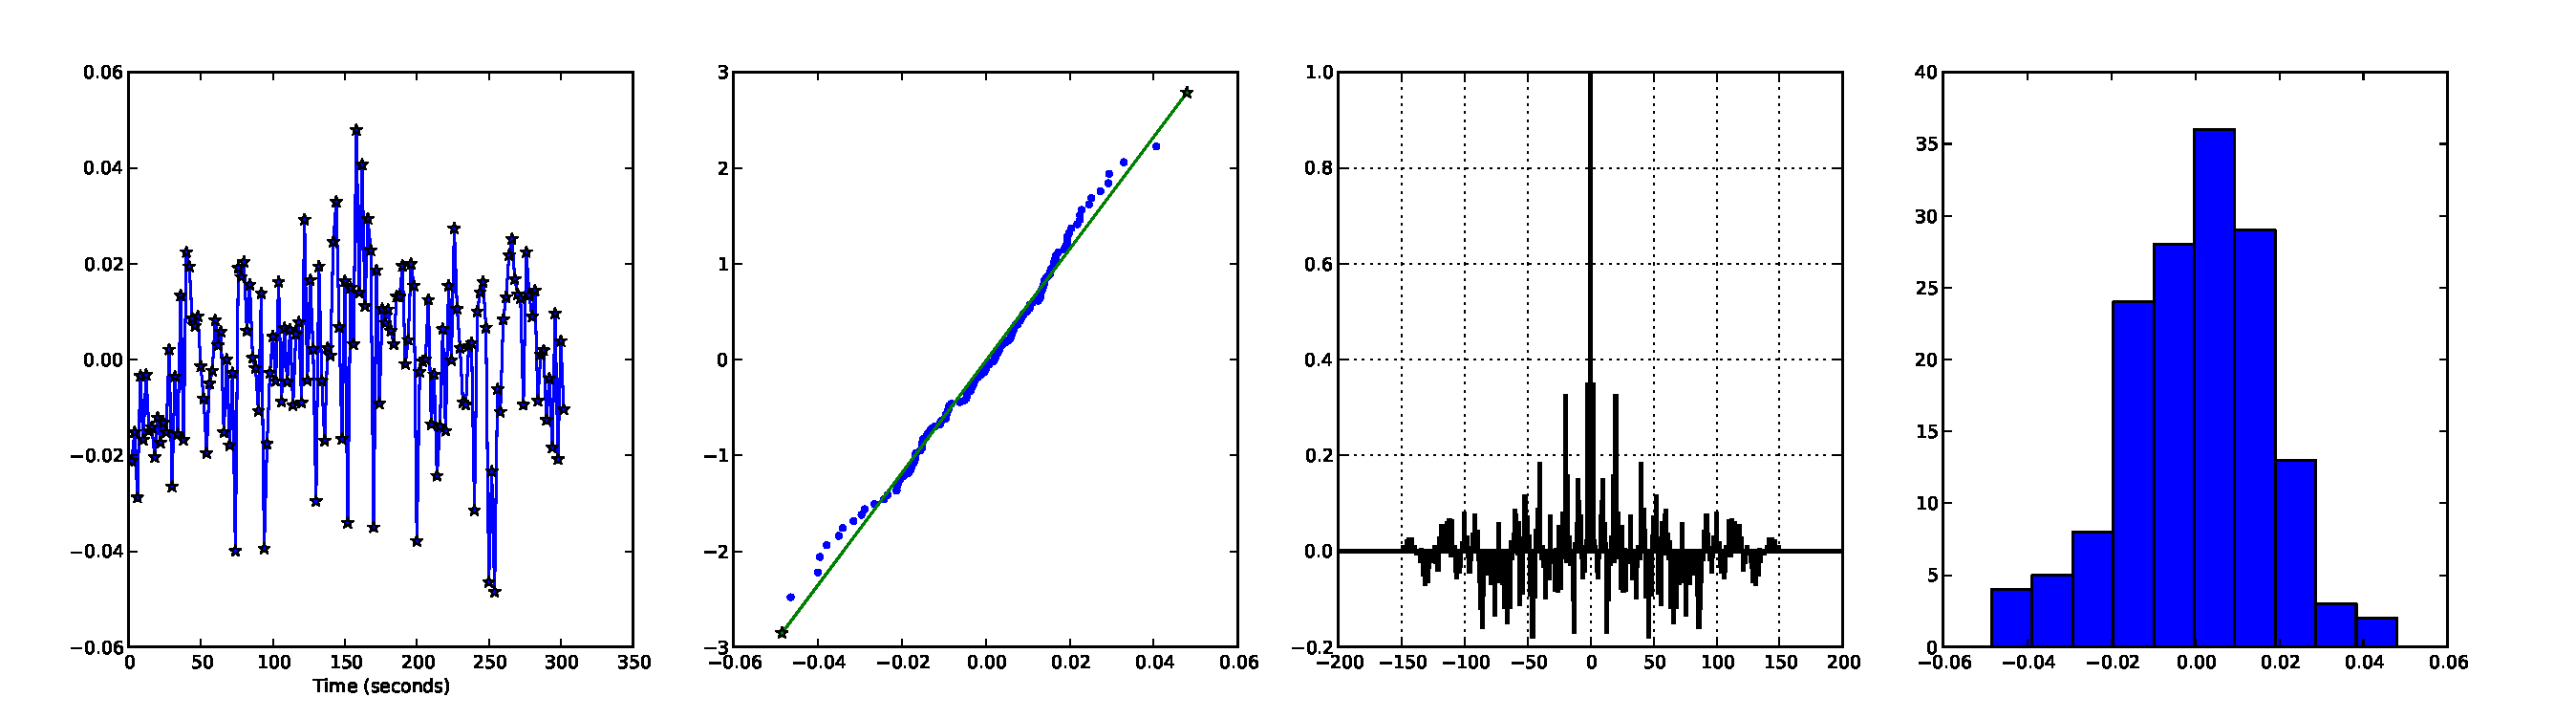
\includegraphics[trim=6cm 1cm 6cm 0cm,width=14cm]{images/noise2_0009_29_49_9}}
\subfigure[]{\label{fig:QQDC:B}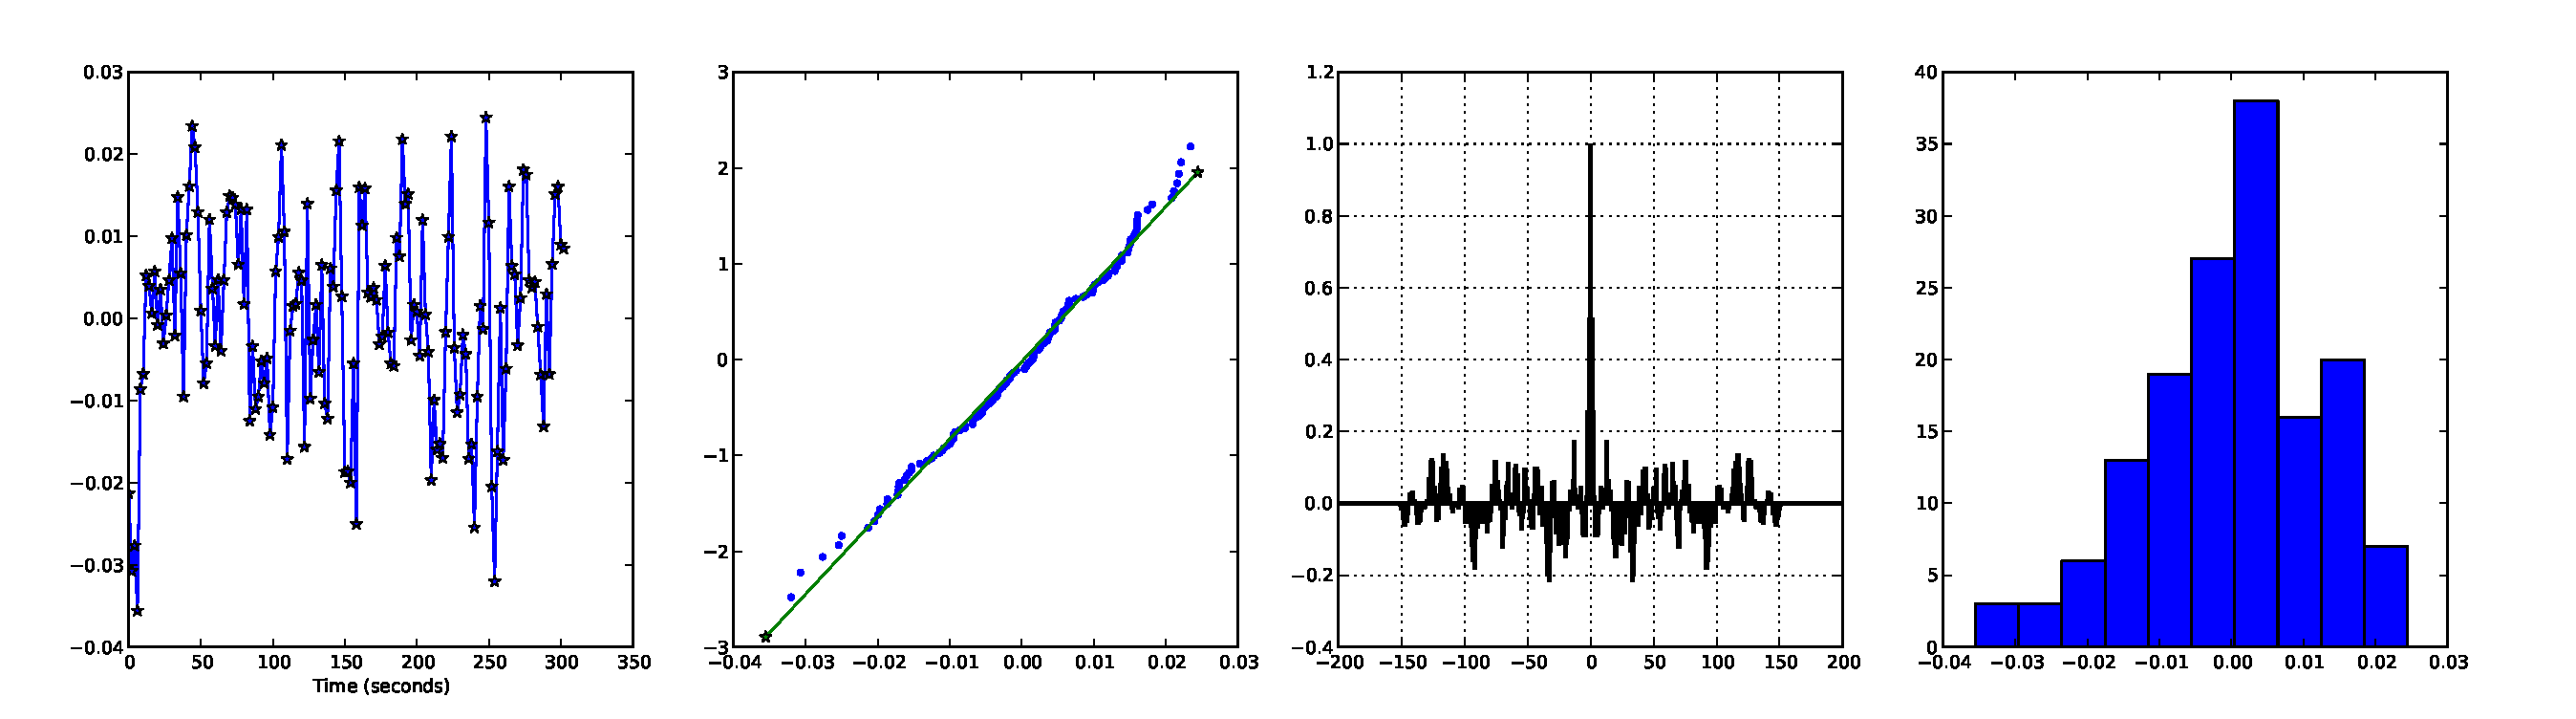
\includegraphics[trim=6cm 1cm 6cm 0cm,width=14cm]{images/noise2_0009_34_43_24}}
\subfigure[]{\label{fig:QQDC:C}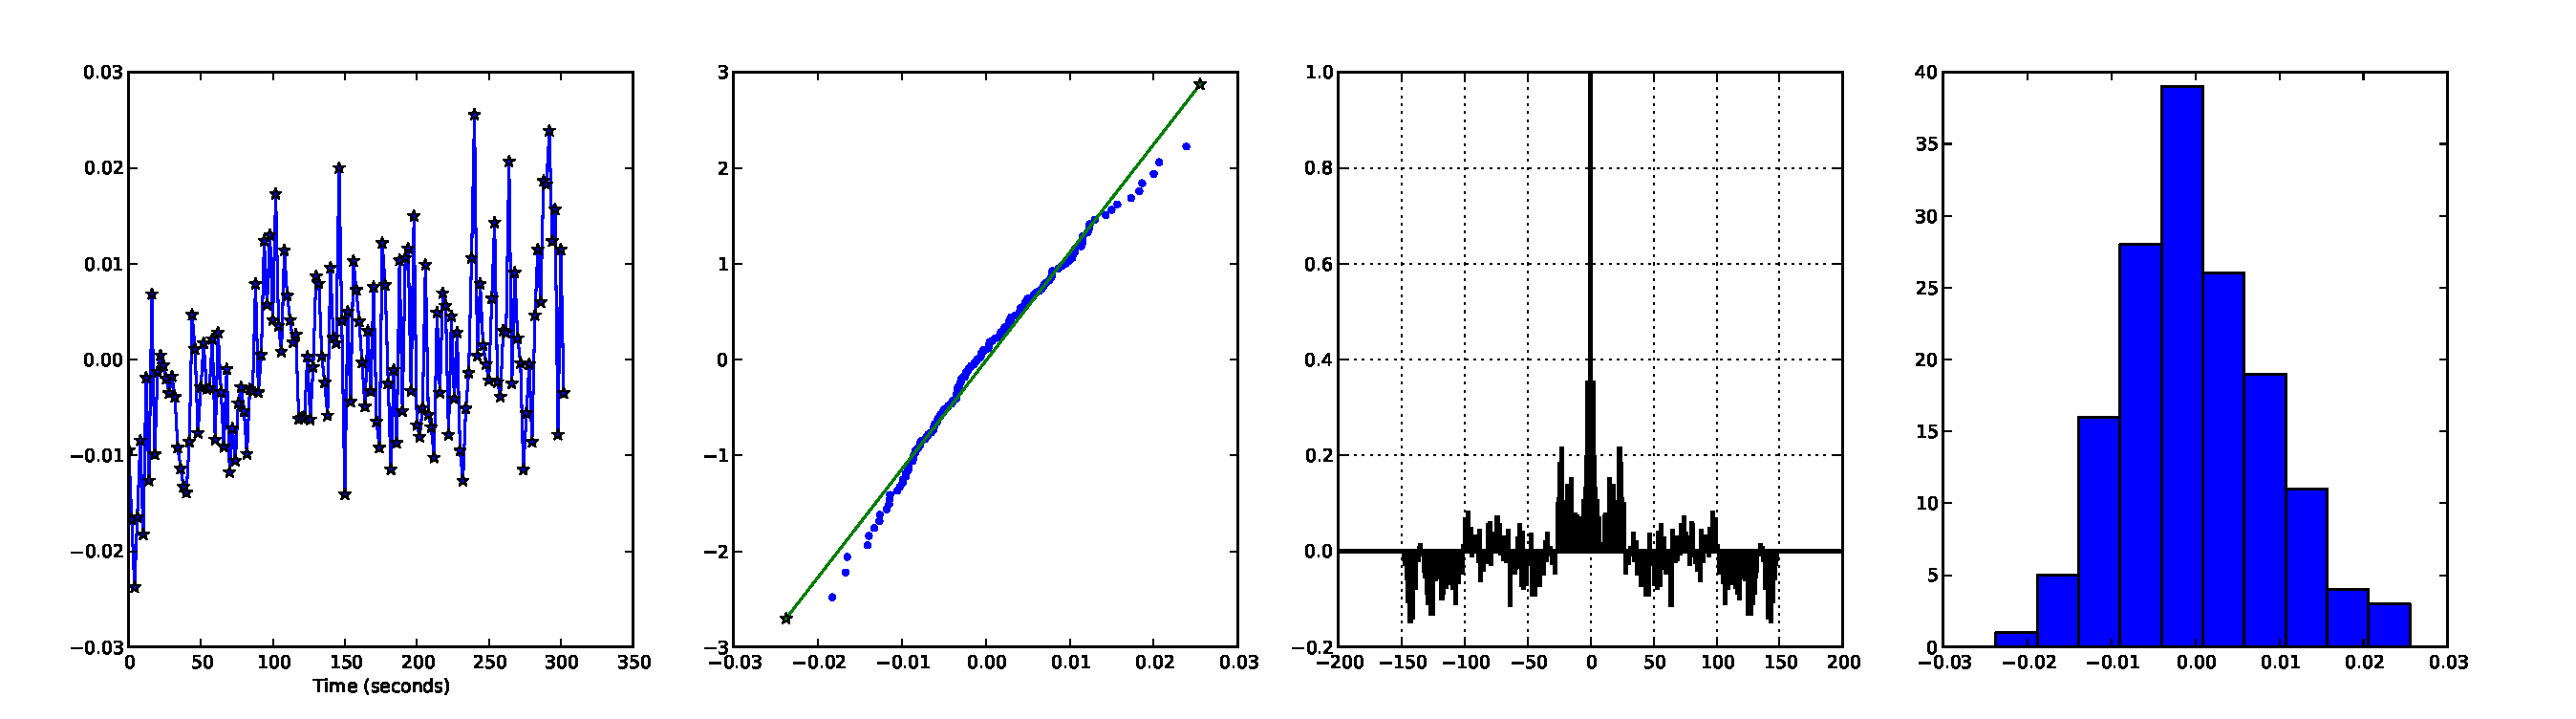
\includegraphics[trim=6cm 1cm 6cm 0cm,width=14cm]{images/noise2_0009_22_38_23}}
\subfigure[]{\label{fig:QQDC:D}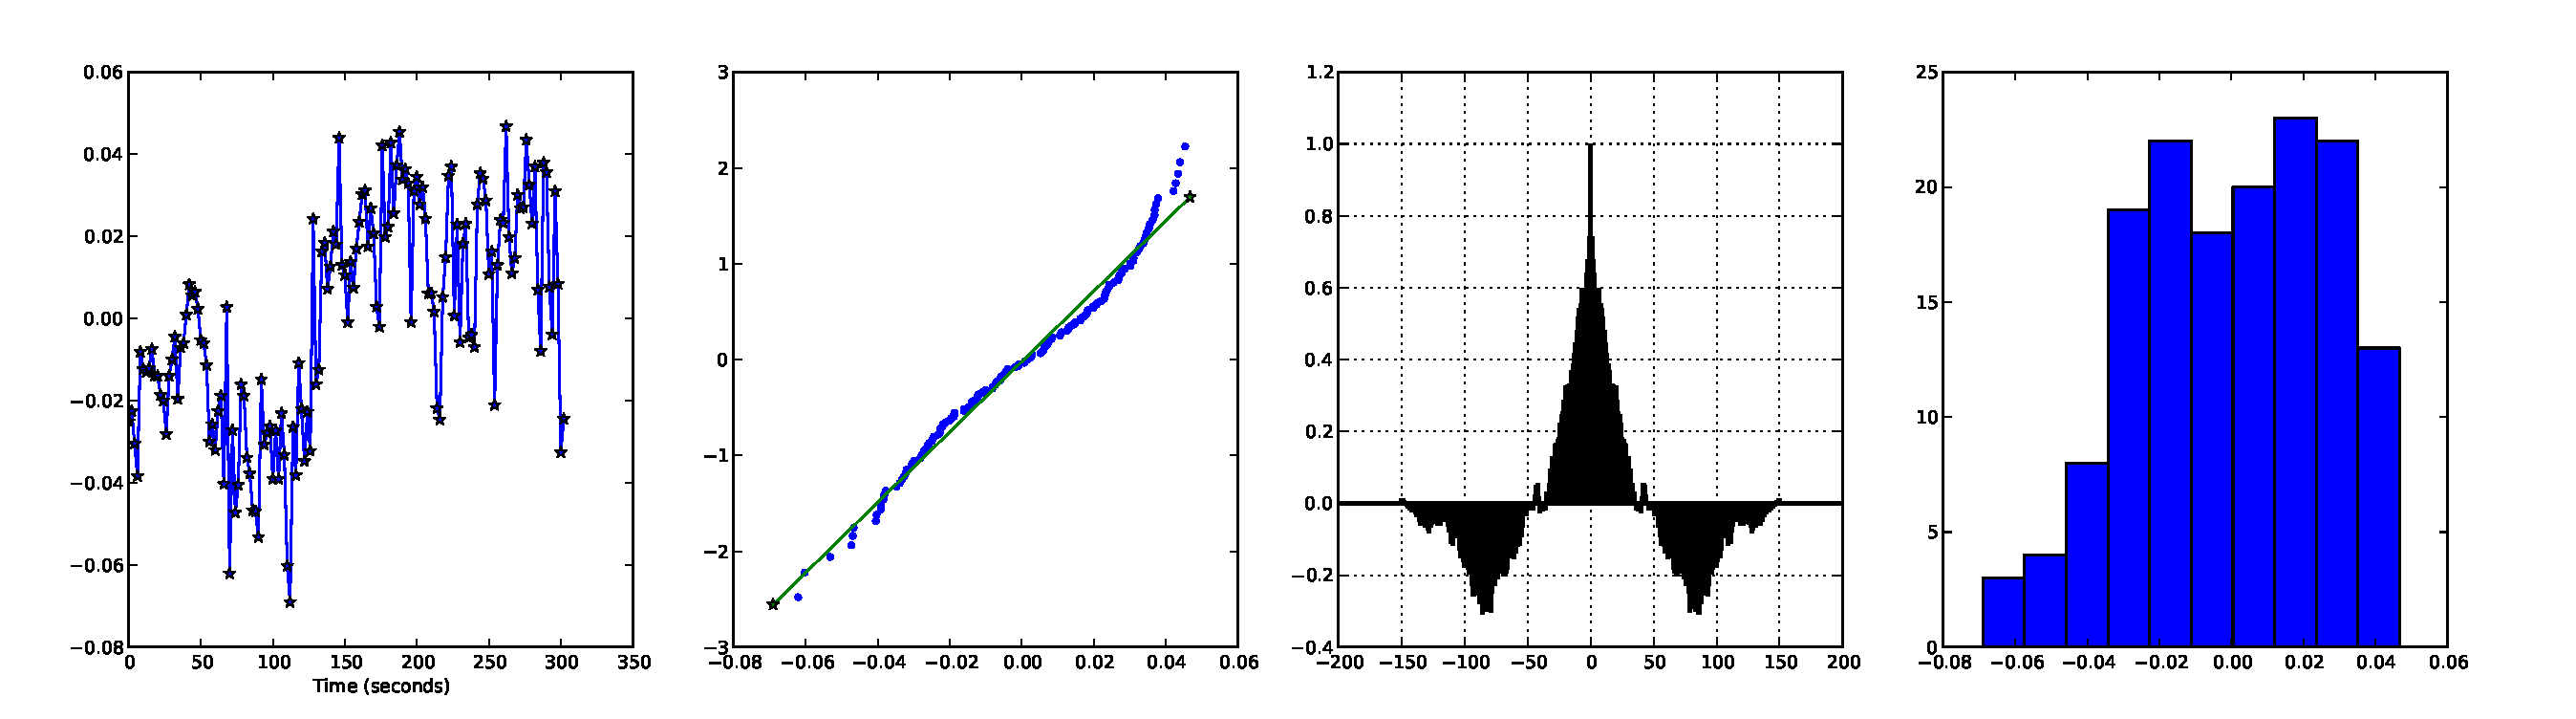
\includegraphics[trim=6cm 1cm 6cm 0cm,width=14cm]{images/noise2_0009_37_29_24}}

%\subfigure{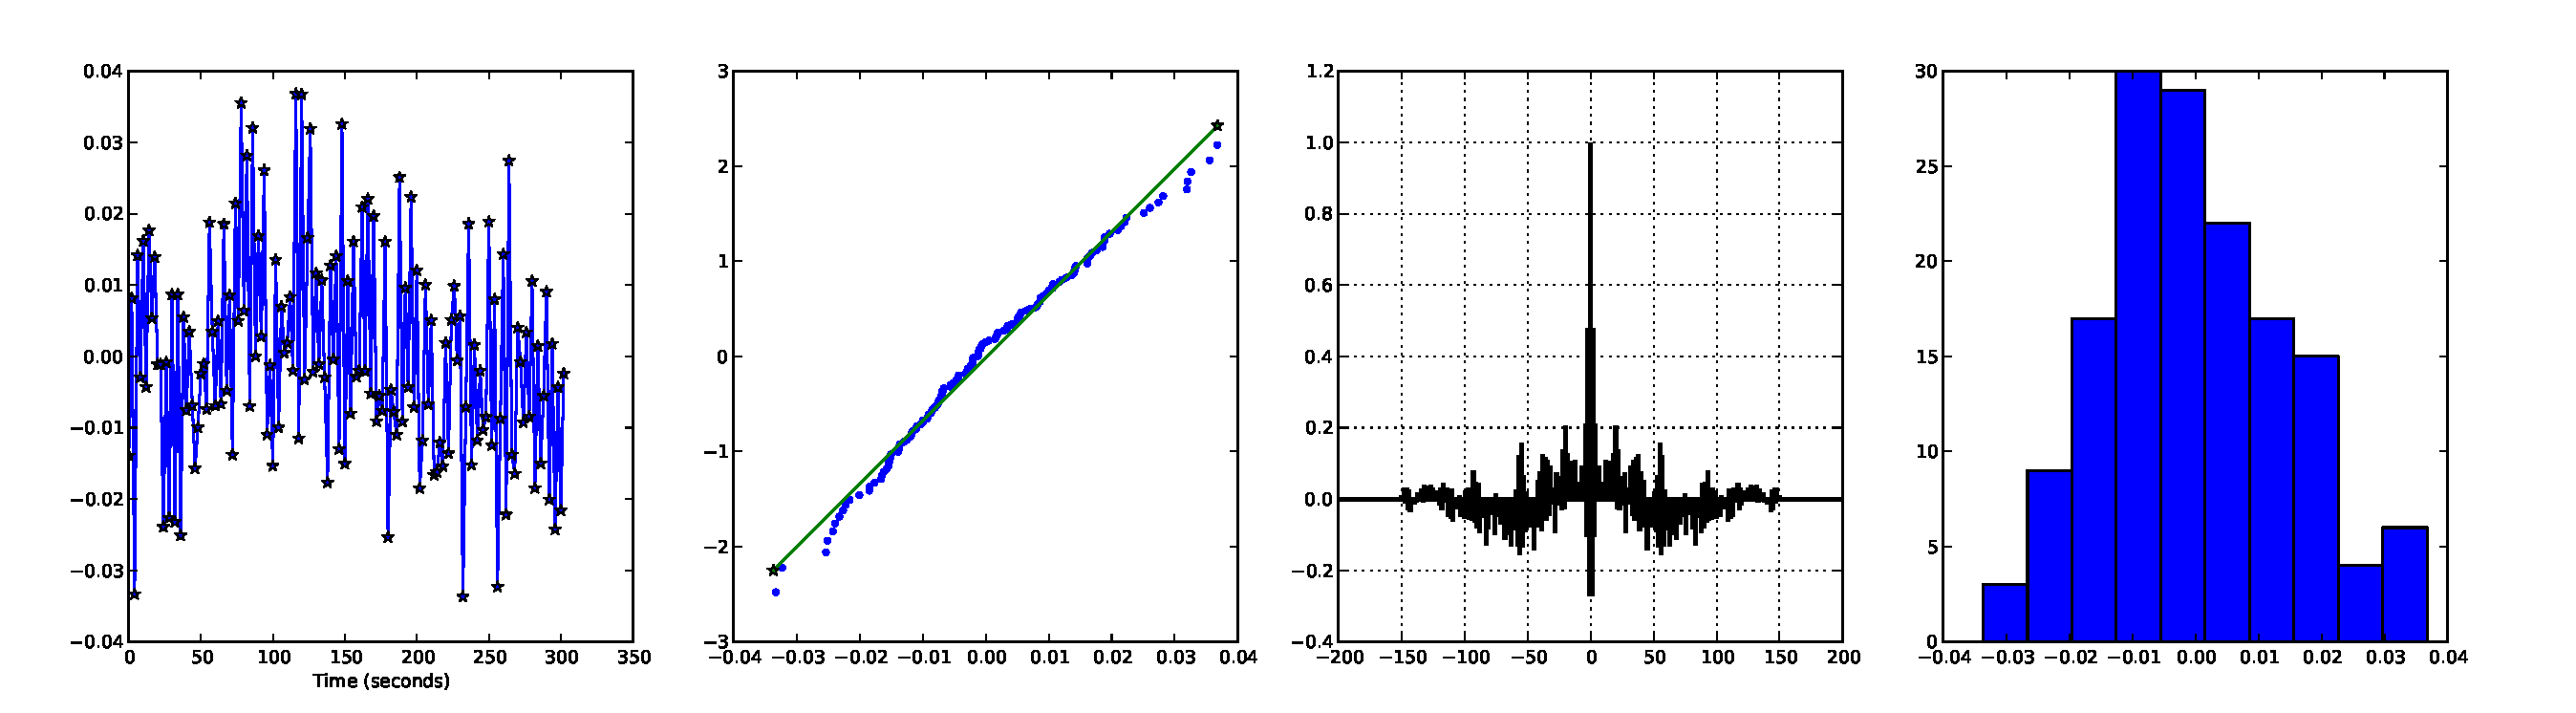
\includegraphics[trim=6cm 1cm 0 0cm,width=17cm]{images/noise_0009_19-24-10.pdf}}
%\subfigure{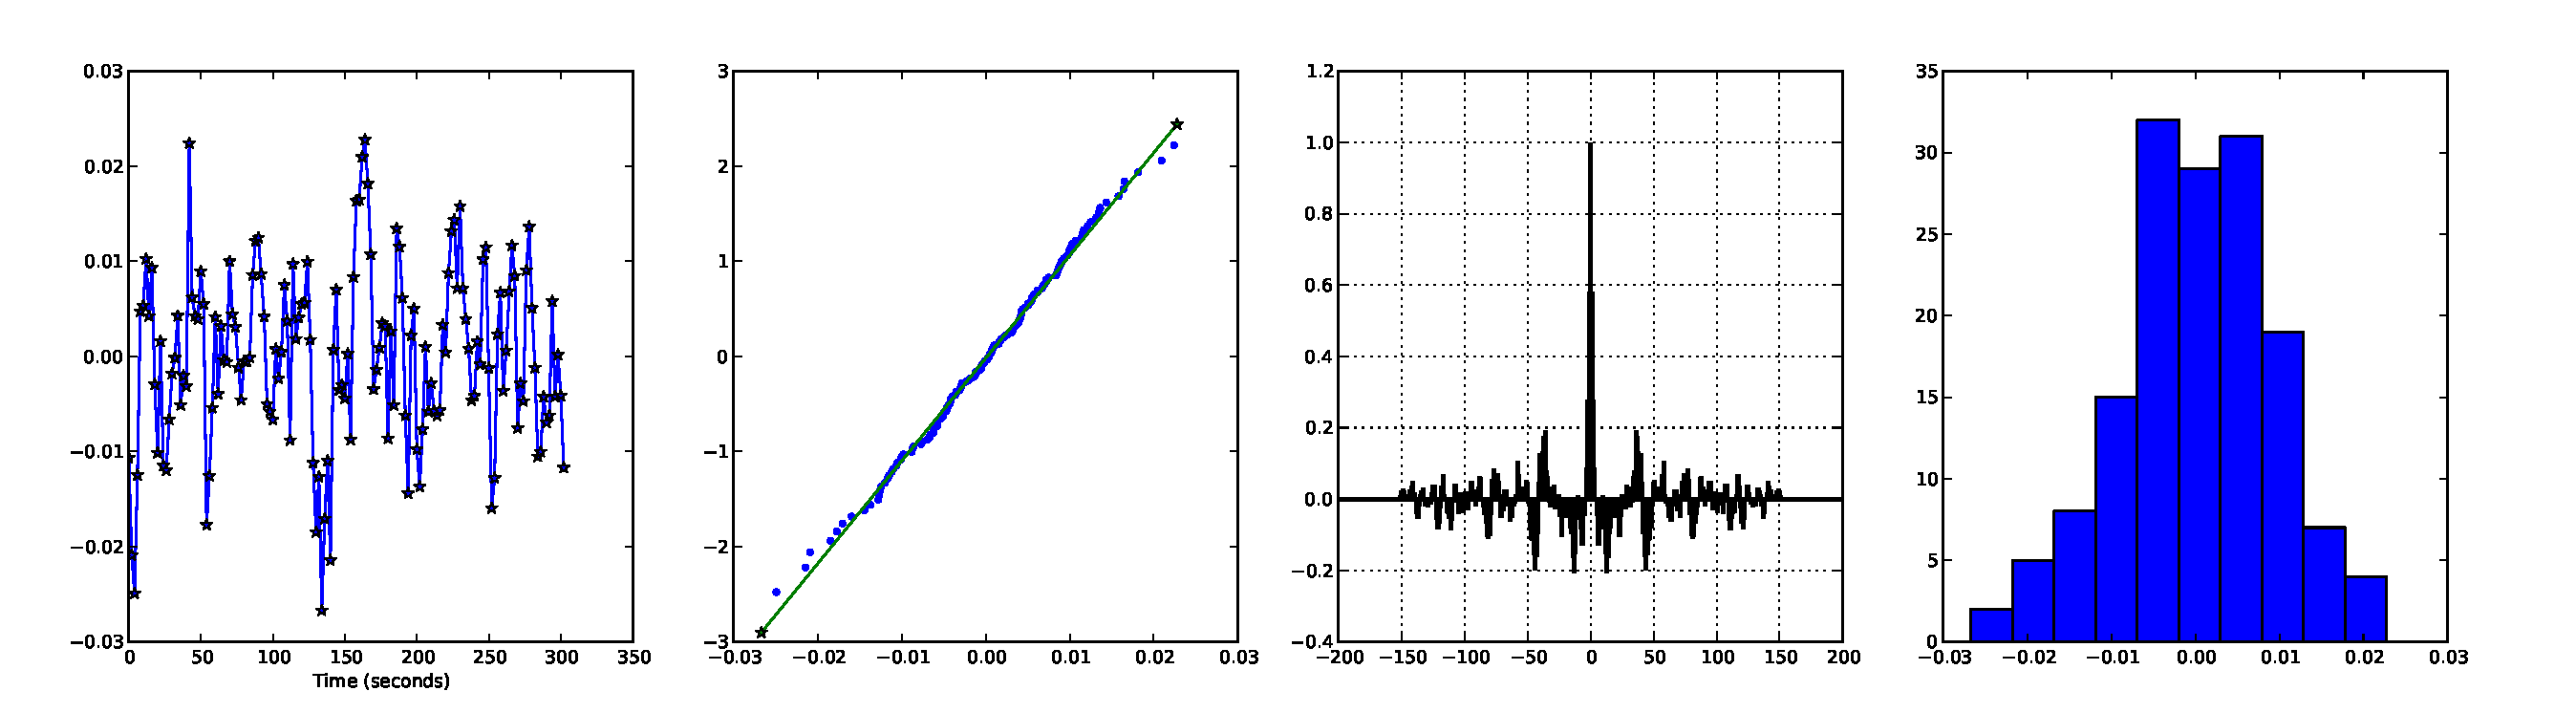
\includegraphics[trim=6cm 1cm 0 0cm,width=17cm]{images/noise_0009_20-45-18.pdf}}
%\subfigure{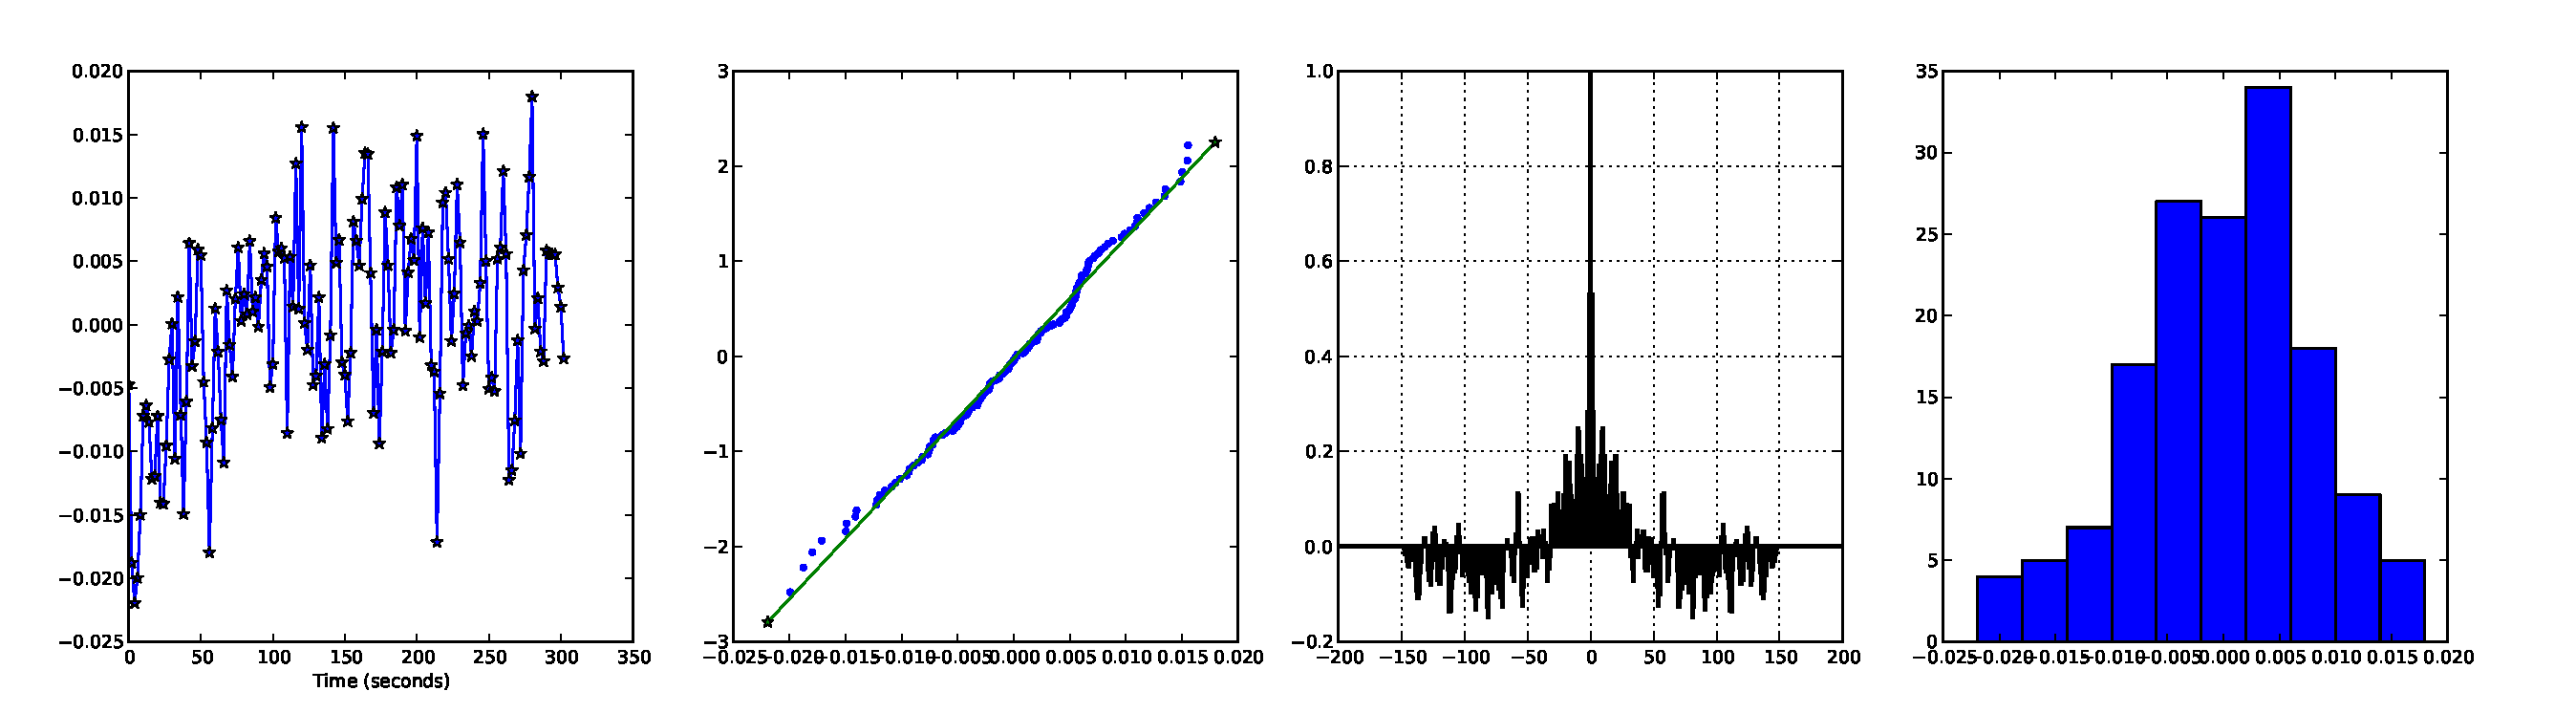
\includegraphics[trim=6cm 1cm 0 0cm,width=17cm]{images/noise_0009_23-47-18.pdf}}
%\subfigure{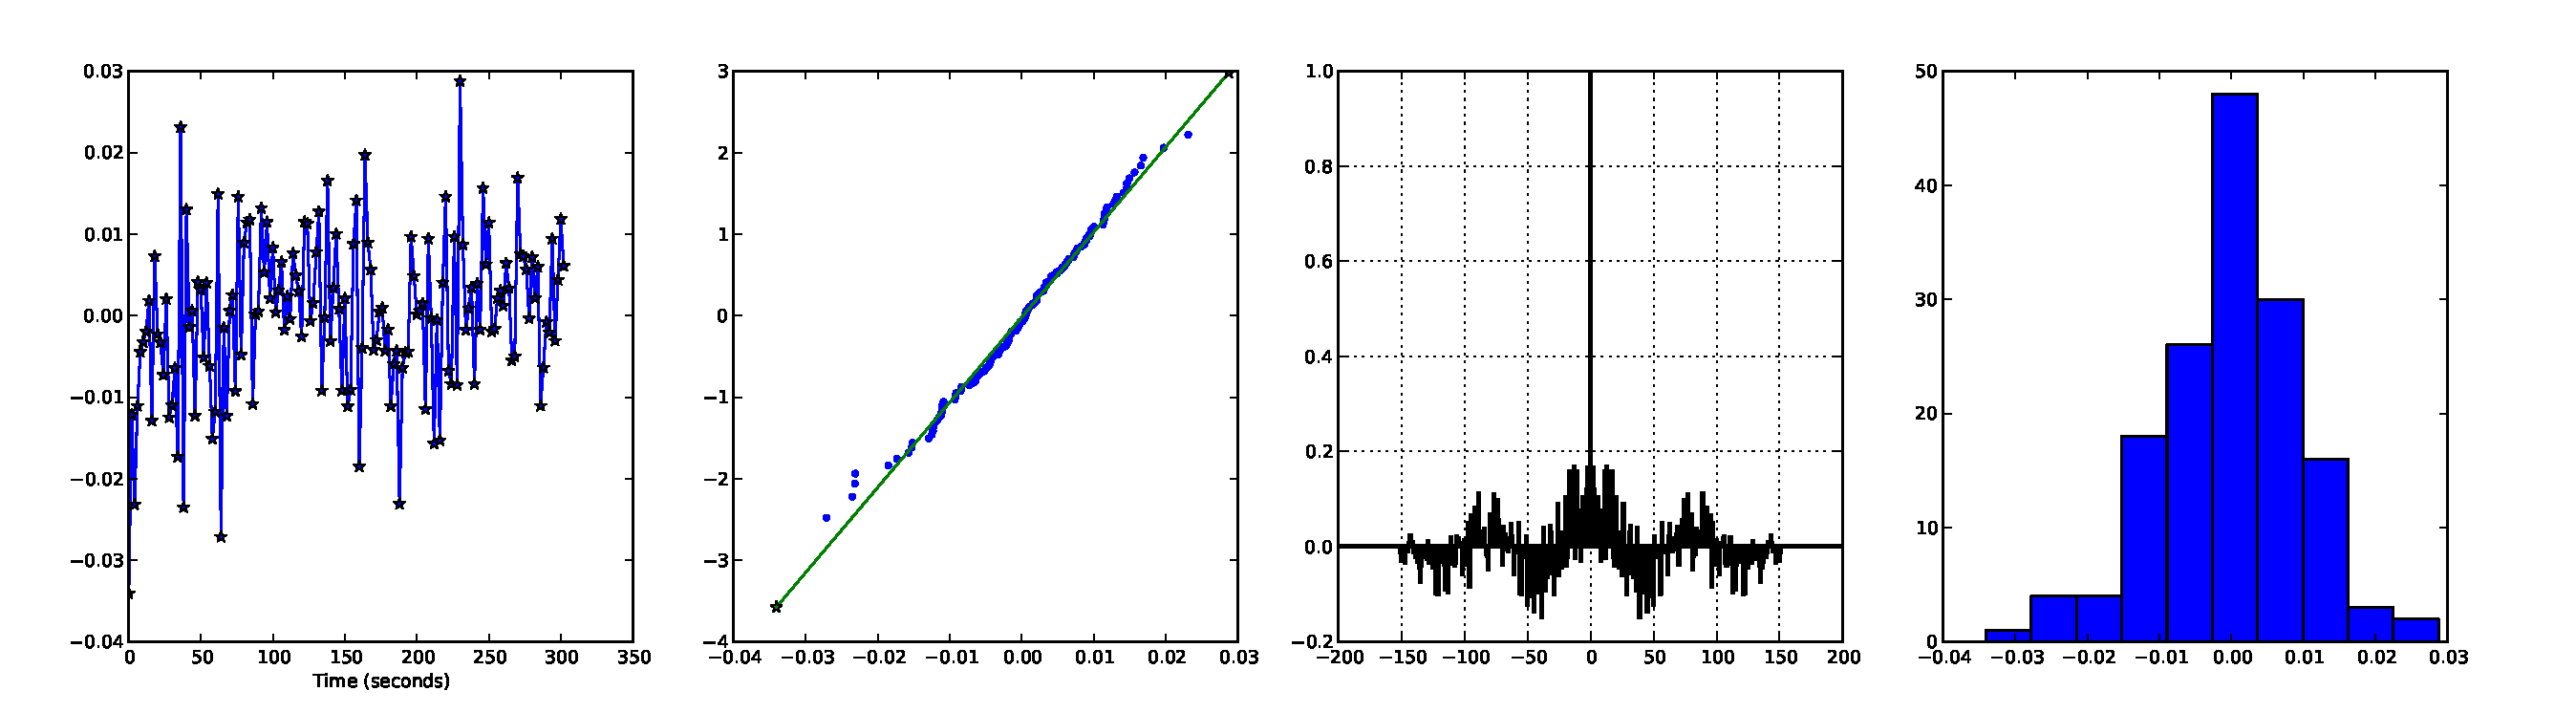
\includegraphics[trim=6cm 1cm 0 0cm,width=17cm]{images/noise_0009_35-49-9.pdf}}

\caption{Q-Q Plots of normalized resting state data}
\label{fig:QQDC}
\end{figure}

\begin{figure}
\centering
\subfigure[]{\label{fig:QQDDlta:A}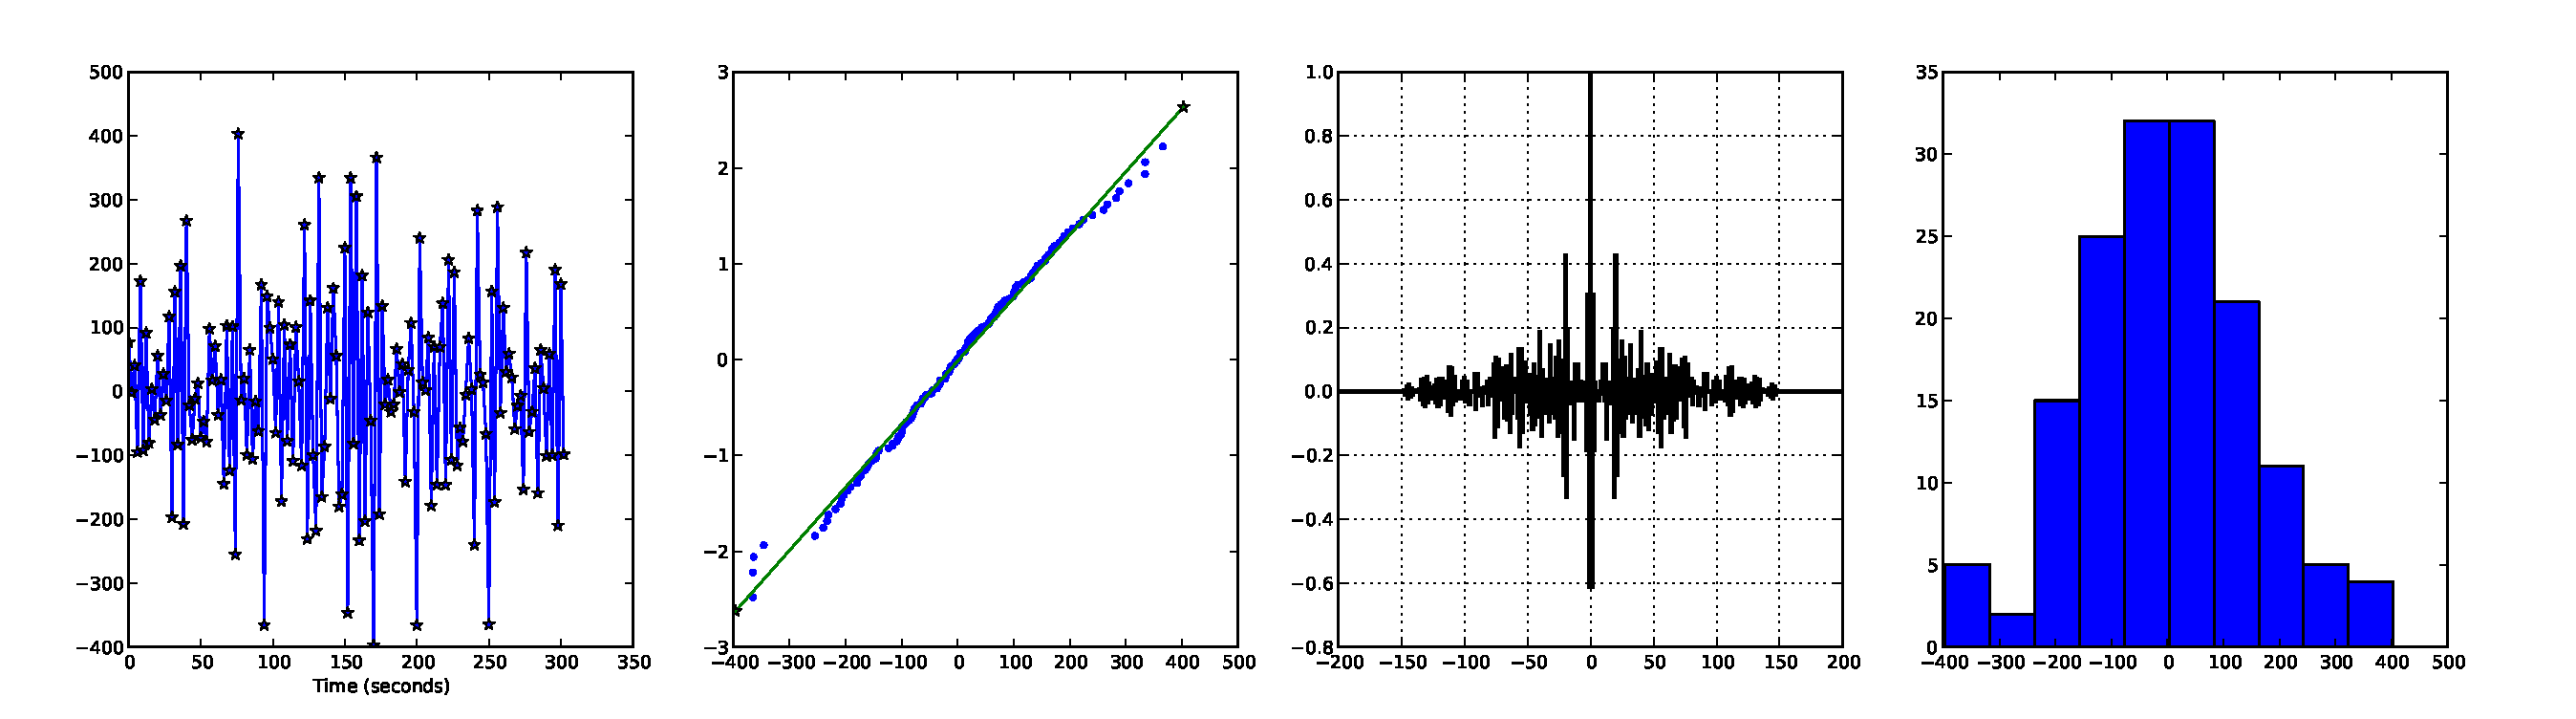
\includegraphics[trim=6cm 1cm 6cm 0,width=14cm]{images/noise2_0009d_29_49_9}}
\subfigure[]{\label{fig:QQDDlta:B}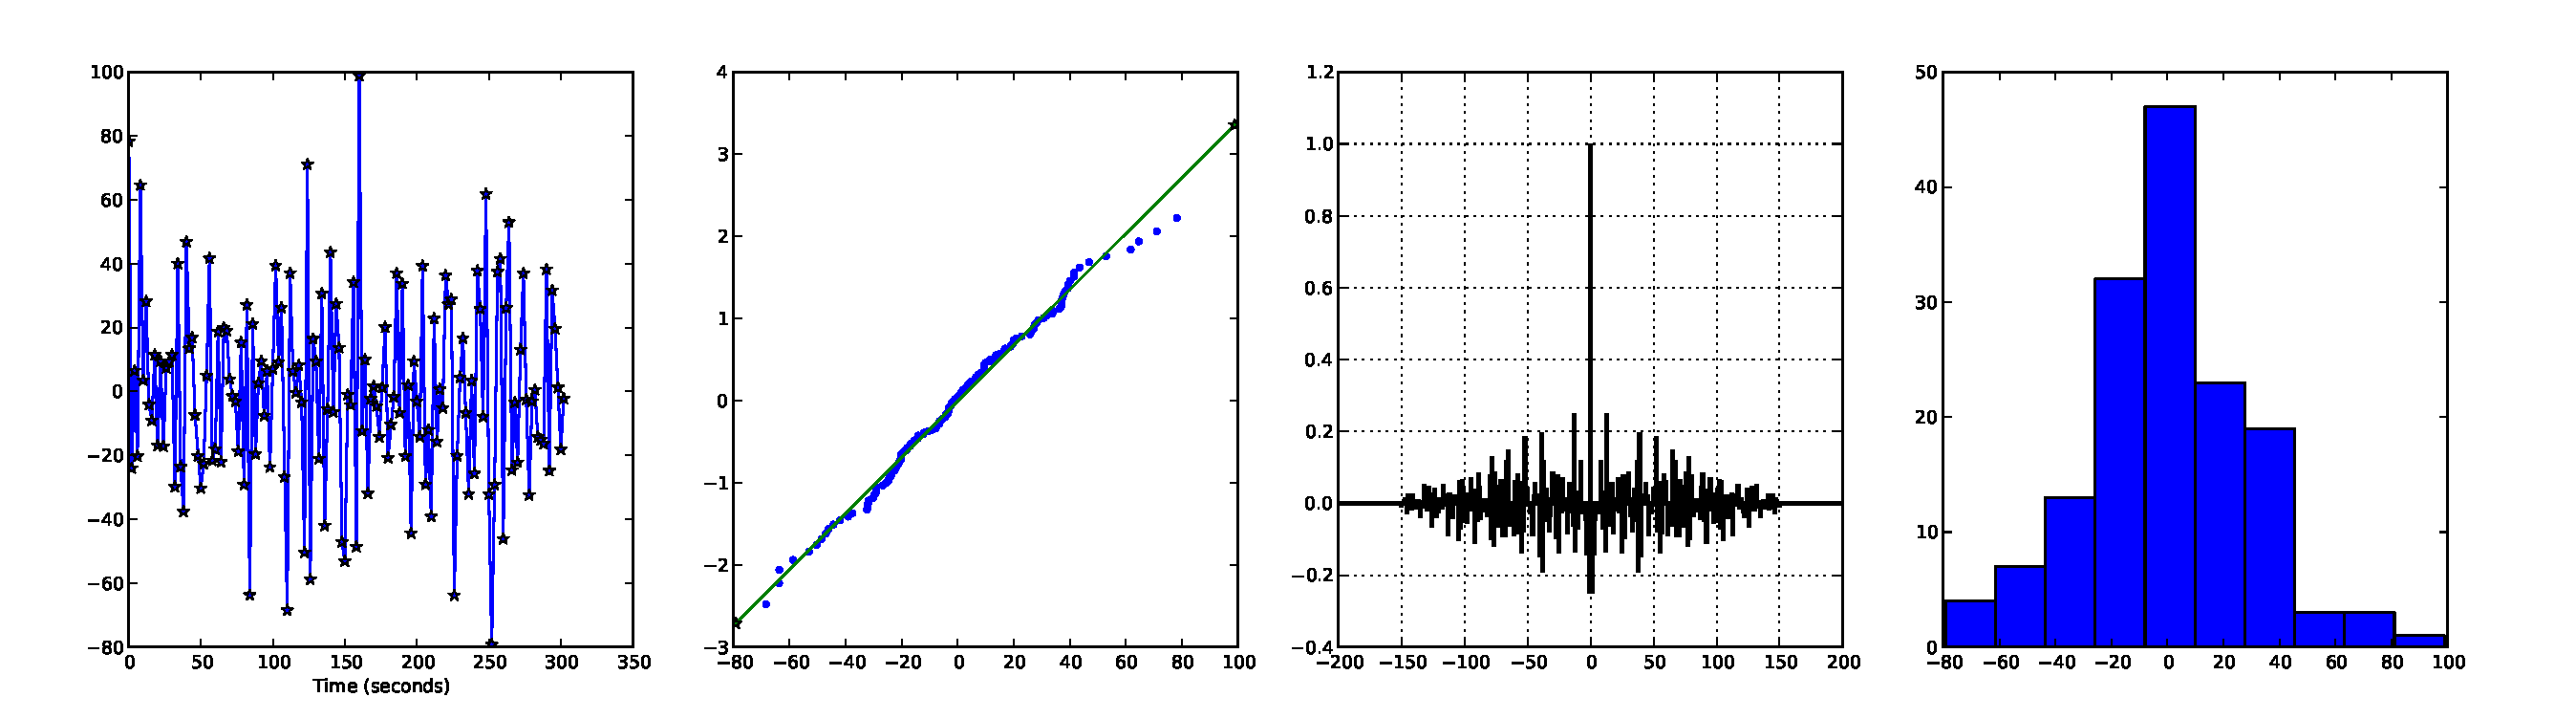
\includegraphics[trim=6cm 1cm 6cm 0,width=14cm]{images/noise2_0009d_34_43_24}}
\subfigure[]{\label{fig:QQDelta:C}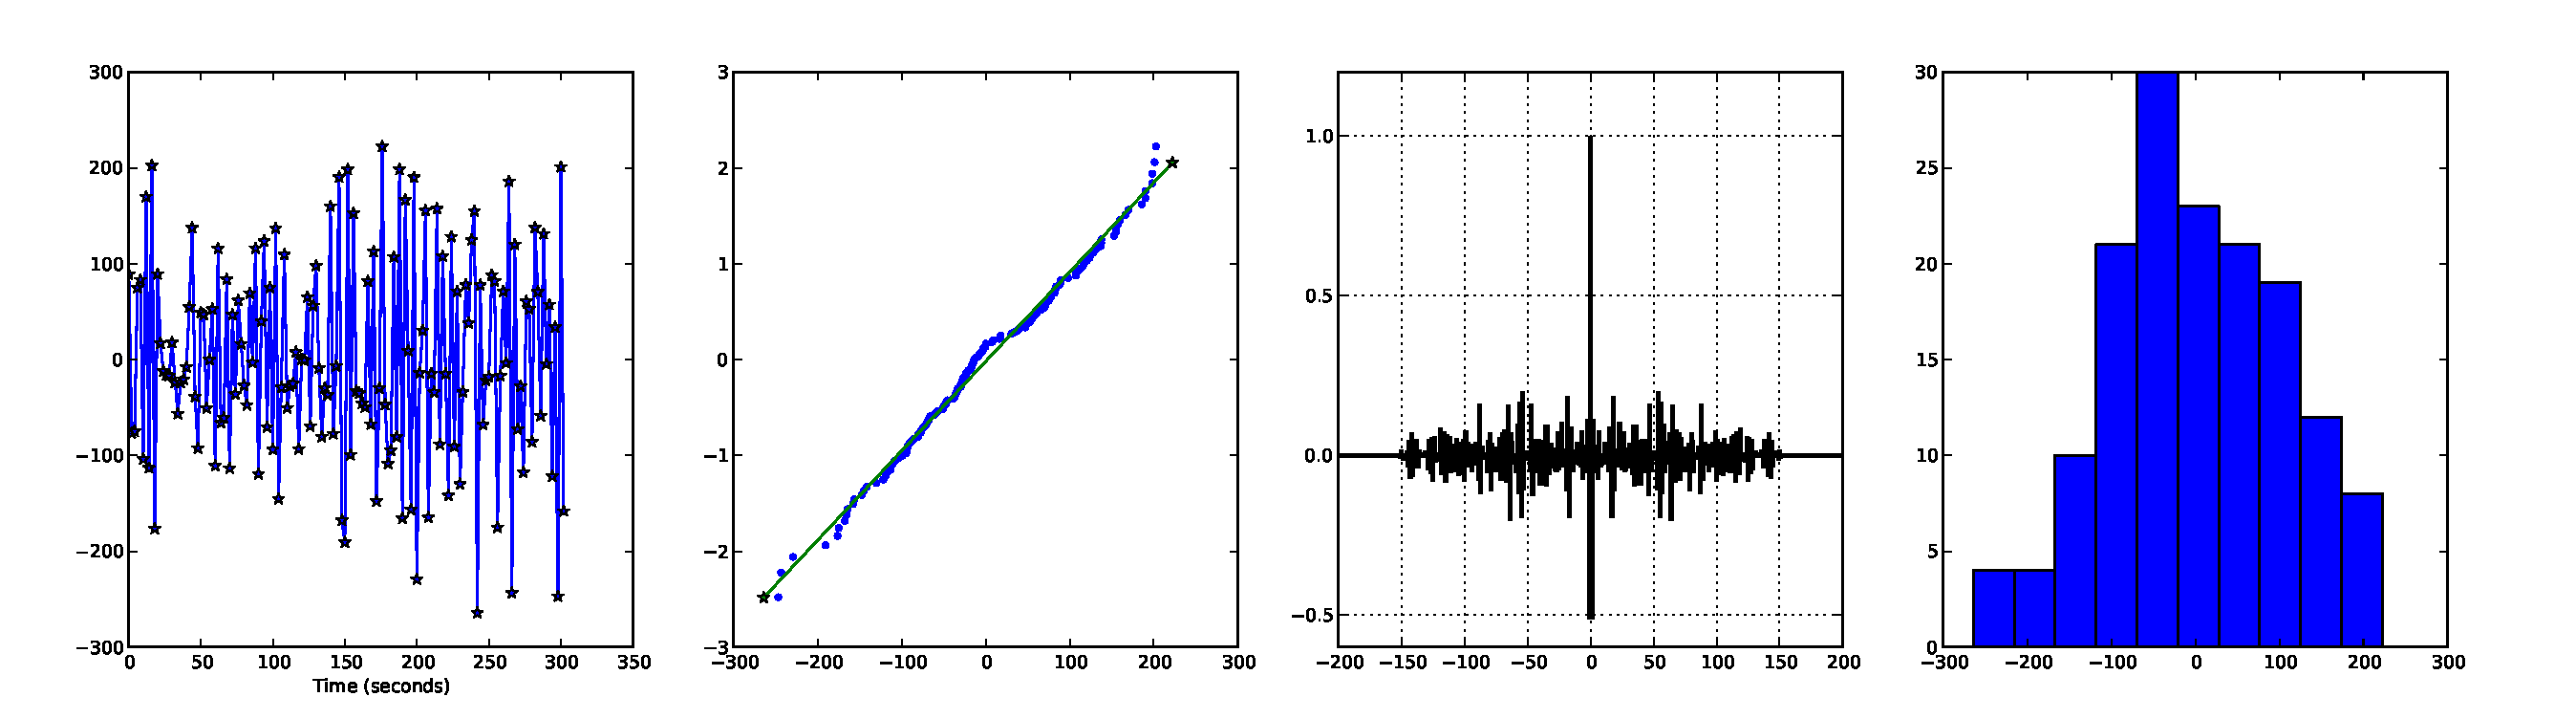
\includegraphics[trim=6cm 1cm 6cm 0,width=14cm]{images/noise2_0009d_22_38_23}}
\subfigure[]{\label{fig:QQDDlta:D}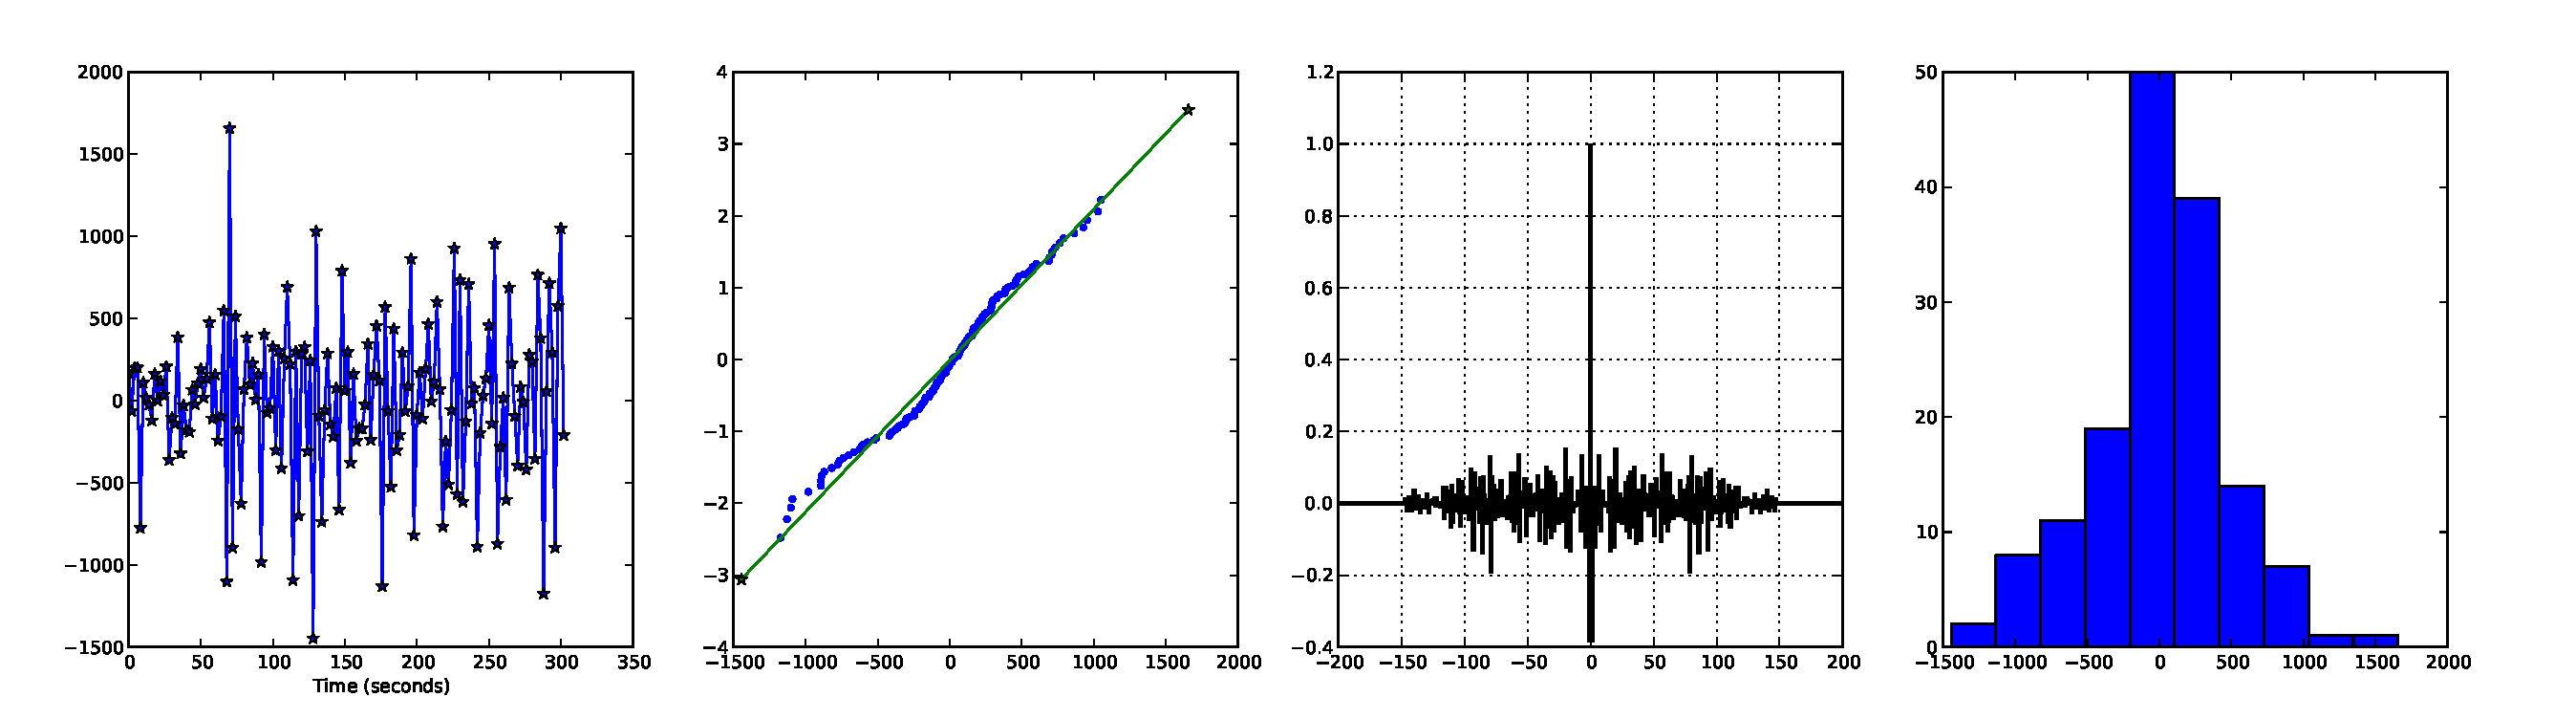
\includegraphics[trim=6cm 1cm 6cm 0,width=14cm]{images/noise2_0009d_37_29_24}}
\caption{Q-Q Plots of resting state data, using the BOLD signal changes}
\label{fig:QQDelta}
\end{figure}

A Wiener process should still conform to the normal distribution, albeit with a 
variance proportional to the run-time. Note that \autoref{fig:QQDC:A} and \autoref{fig:QQDC:B}
are relatively well described by a Gaussian process with a small autocorrelation, 
\autoref{fig:QQDC:C} and \autoref{fig:QQDC:D} aren't. In particular the tails don't
seem to fit, which could be well explained by the much more significant drift in the
signal. Thus, its possible a Wiener process does not well describe the error, since overall
the distribution does not tend toward a Gaussian. Still, the steps still seem to
be relatively normal, meaning at the very least that the process is close to Wiener.
As one would expect most of the autocorrelation disappears for the step data, indicating
that the steps are relatively independent. Therefore, the assumption of I.I.D. Normal 
steps is relatively good, even though the accumulated result seems to be less varied than
Wiener.

\begin{figure}
\centering
\subfigure[]{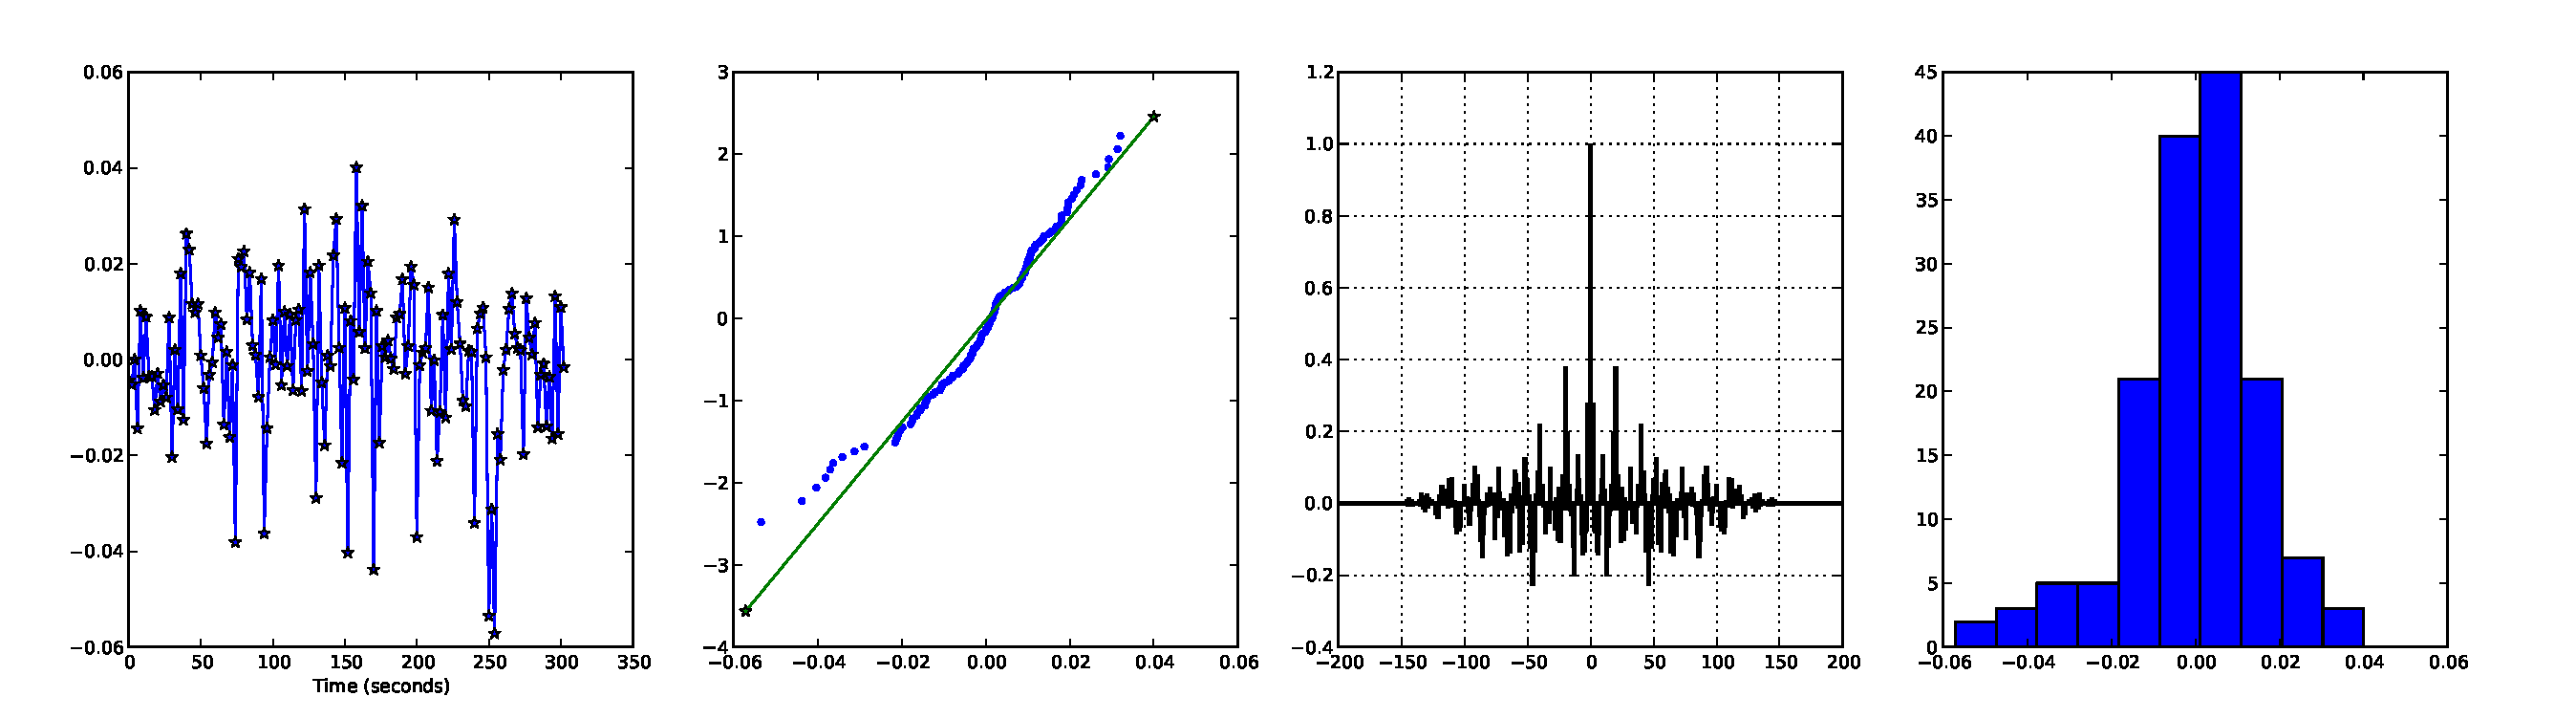
\includegraphics[trim=6cm 1cm 6cm 0cm,width=14cm]{images/noise2_0009s_29_49_9}}
\subfigure[]{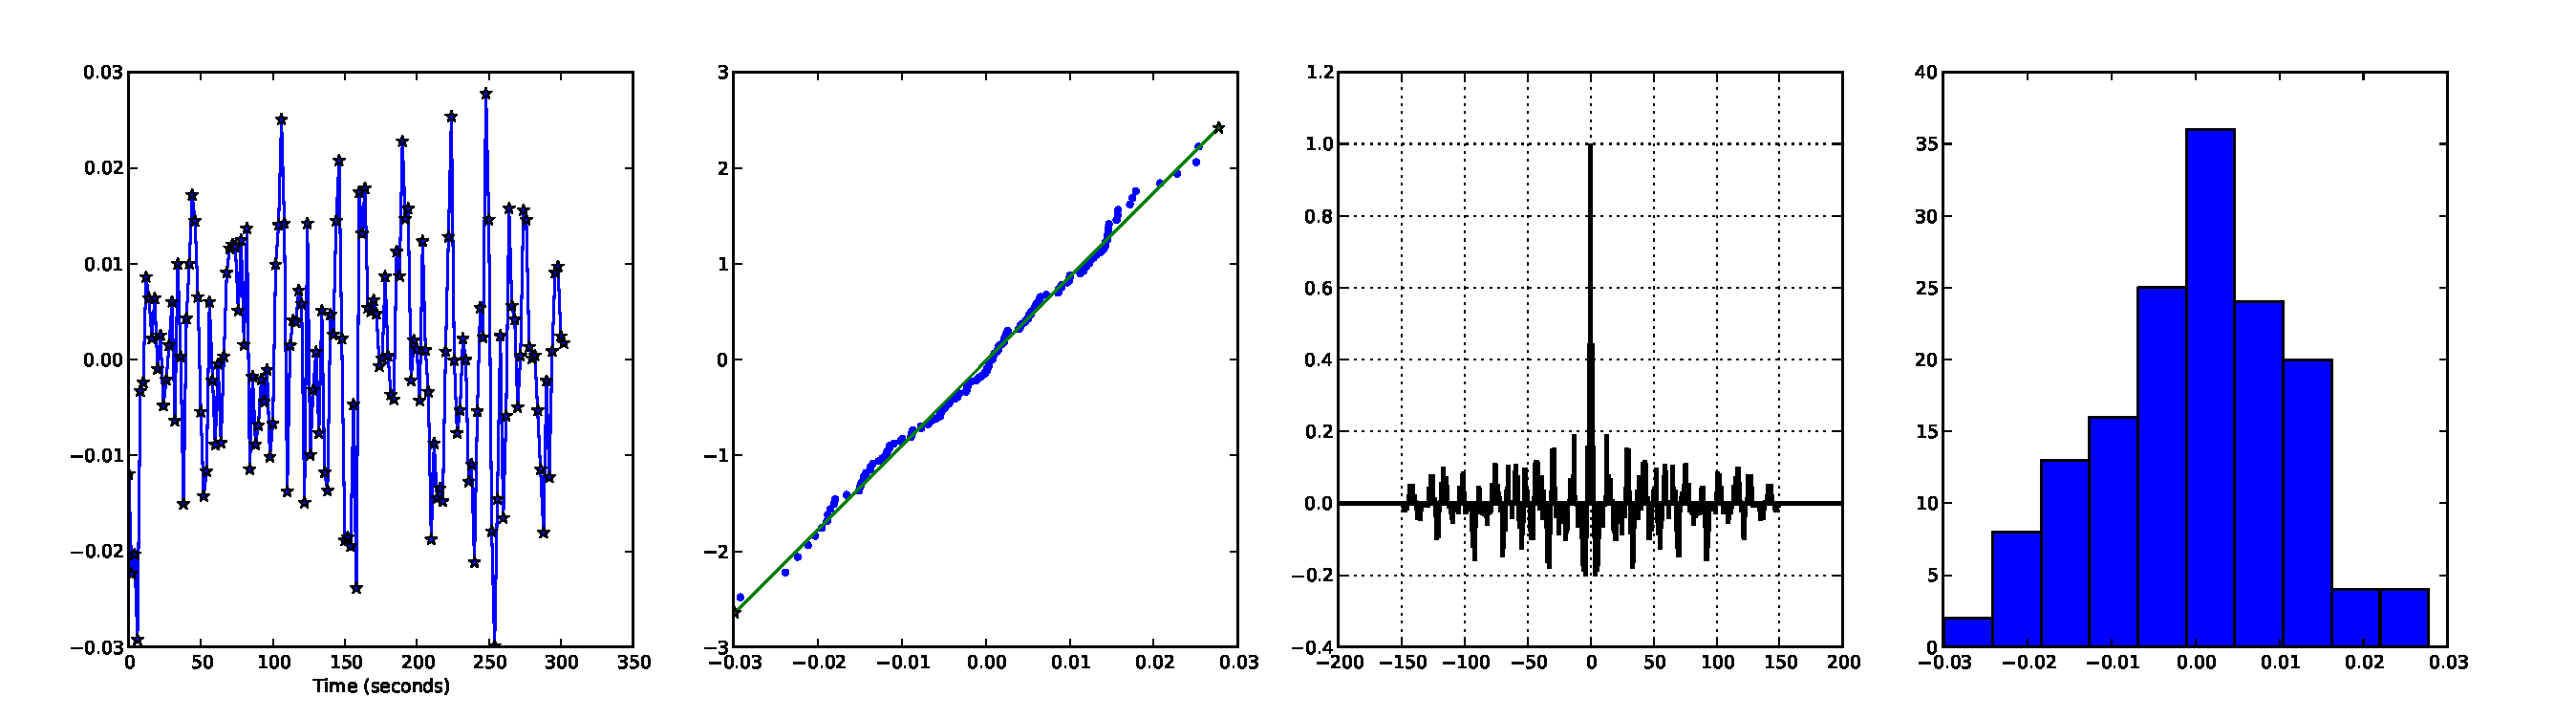
\includegraphics[trim=6cm 1cm 6cm 0cm,width=14cm]{images/noise2_0009s_34_43_24}}
\subfigure[]{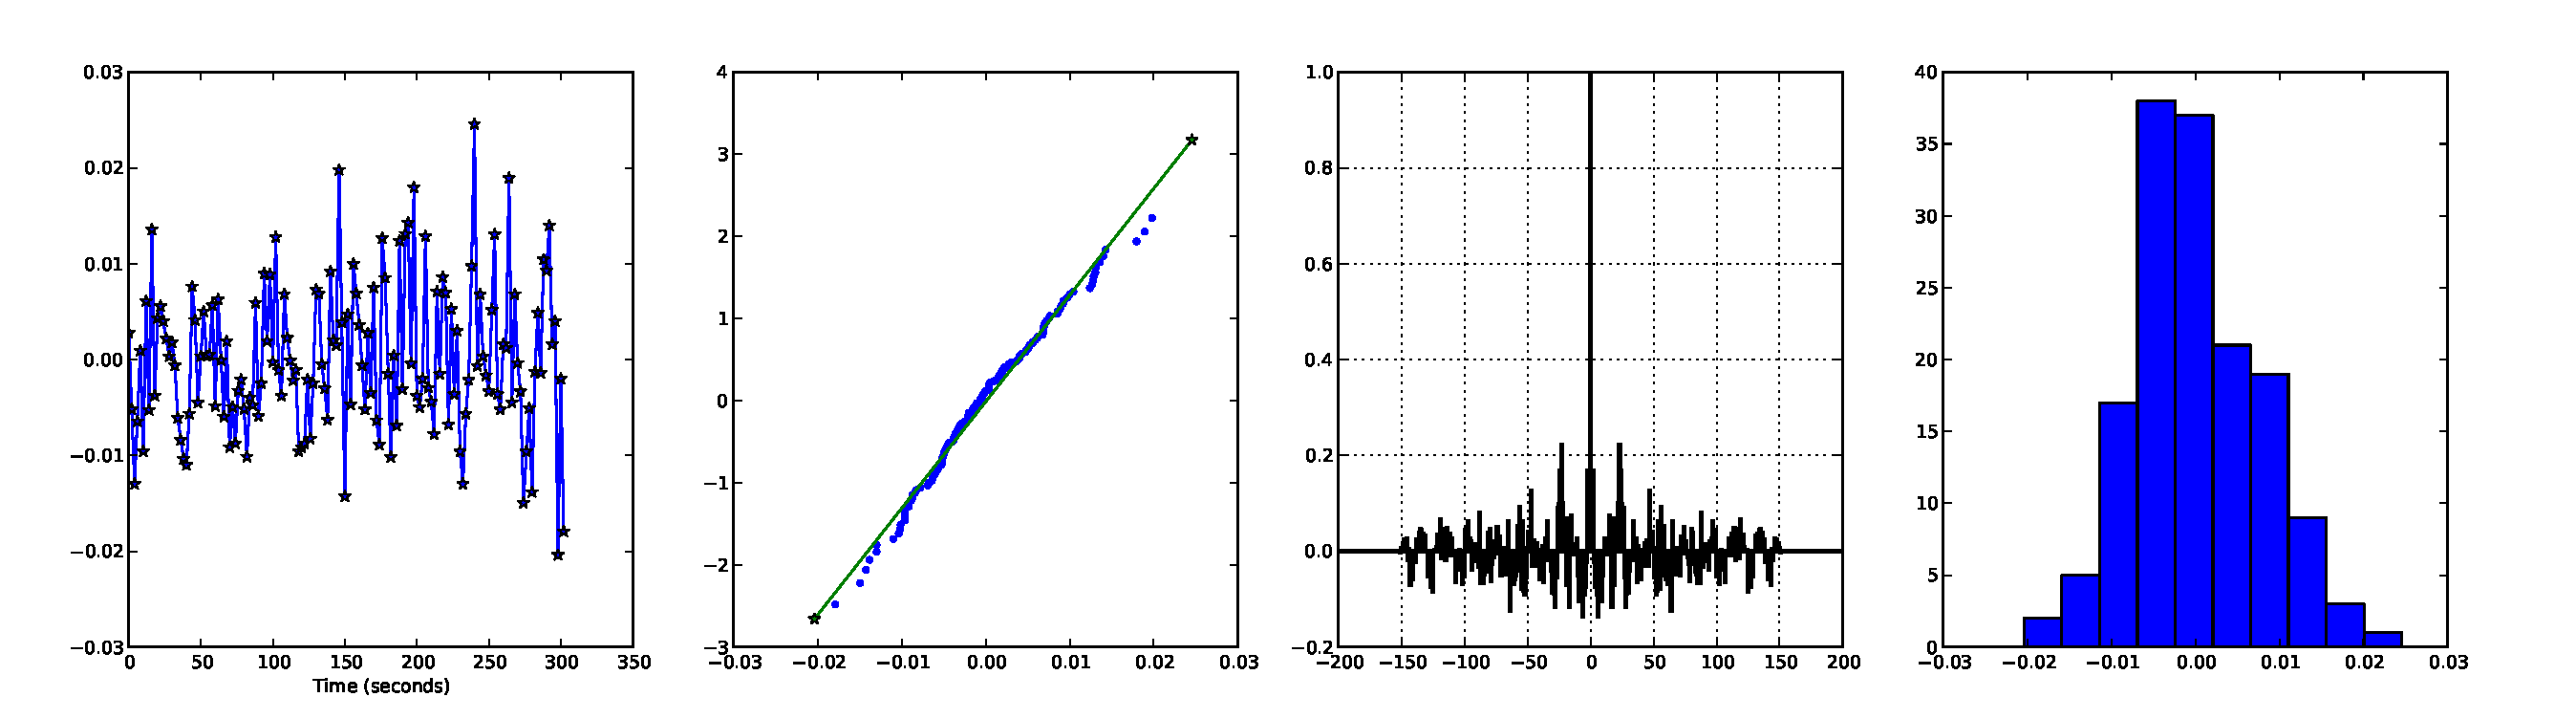
\includegraphics[trim=6cm 1cm 6cm 0cm,width=14cm]{images/noise2_0009s_22_38_23}}
\subfigure[]{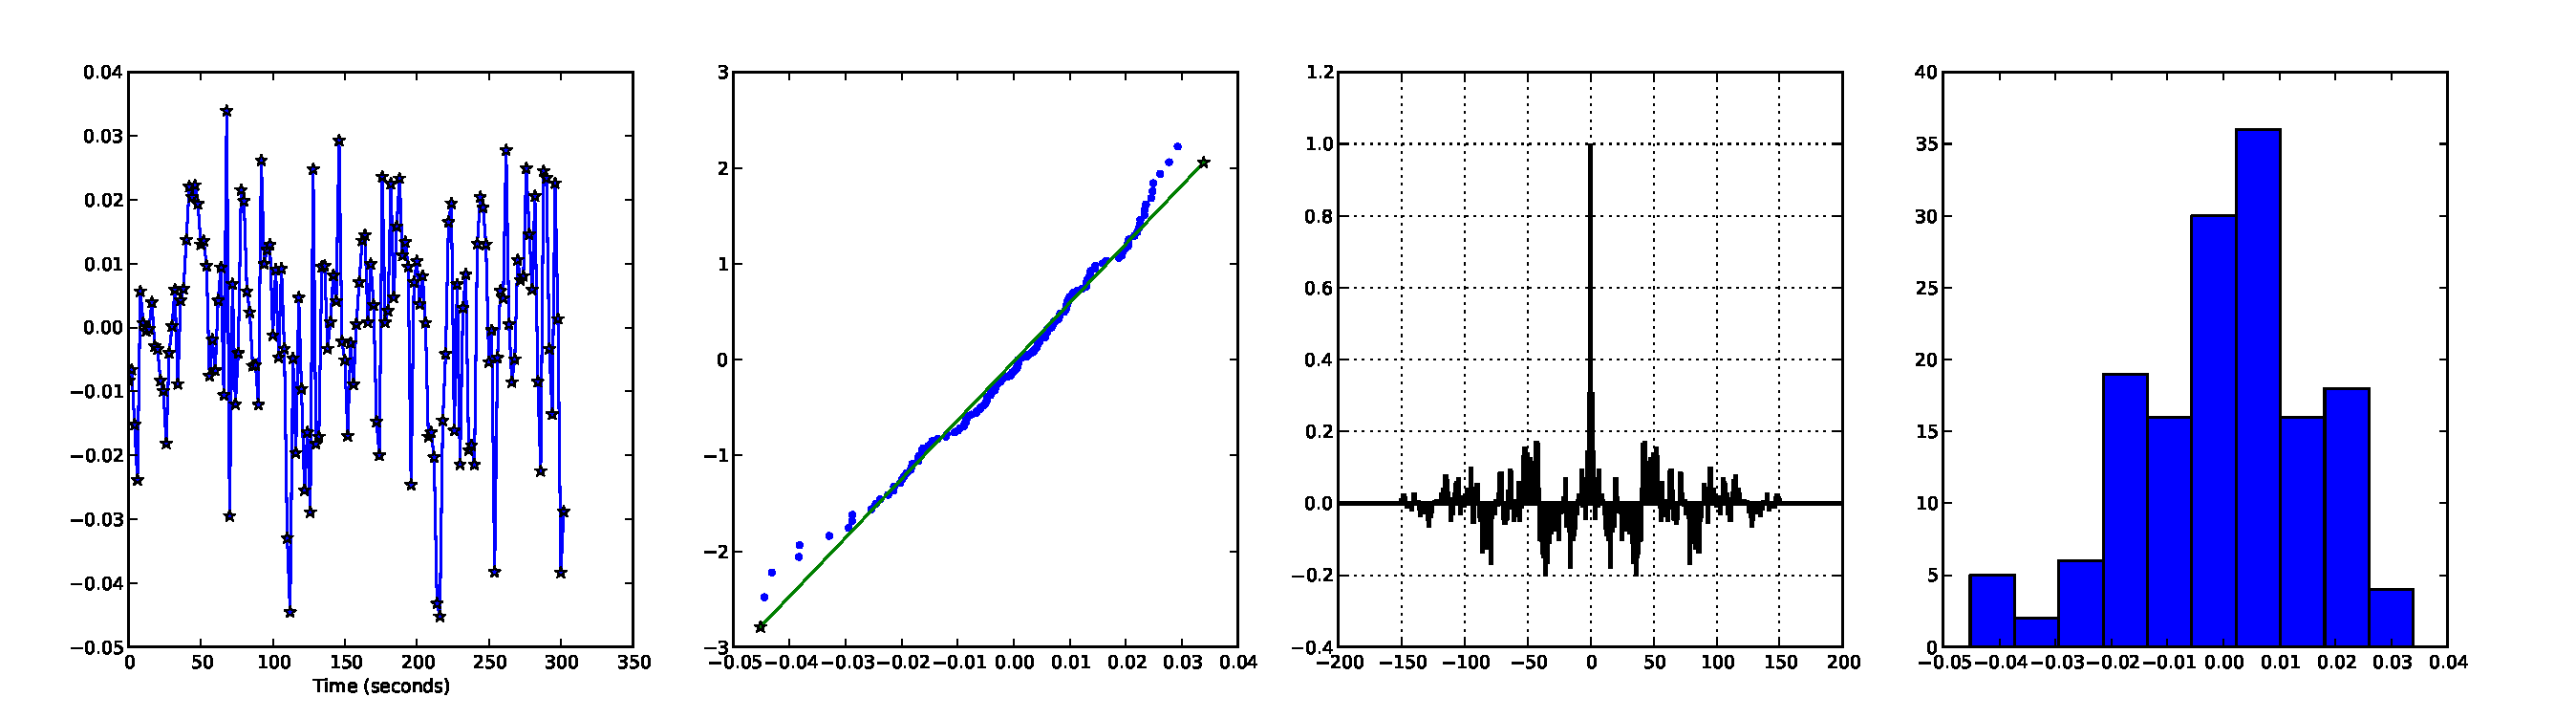
\includegraphics[trim=6cm 1cm 6cm 0cm,width=14cm]{images/noise2_0009s_37_29_24}}
\caption{Q-Q Plots of resting state data, after the de-trending}
\label{fig:QQSpline}
\end{figure}

[todo analysis after detrending]

\section{Analysis of the BOLD Signal}
Several studies have endeavored to analyze the BOLD equations, which
we will review here. The most obvious analysis is to calculate the
steady state signal, when $u$ is held constant long enough for
all the transients to settle out. 

\begin{eqnarray}
s_{ss} &=& 0 \nonumber \\
f_{ss} &=& \tau_f\epsilon u + 1\nonumber \\
v_{ss} &=& (\tau_f\epsilon u + 1)^\alpha\nonumber \\
q_{ss} &=& \frac{(\tau_f\epsilon u + 1)^\alpha}{E_0}(1-(1-E_0)^{1/(\tau_f\epsilon u + 1)})\nonumber \\
y_{ss} &=& V_0((k_1+k_2)(1-q_{ss}) - (k_2+k_3)(1-v_{ss}))
\label{eq:steadystate}
\end{eqnarray}


todo
[Image with two different $\alpha$'s]

[image comparing the results of 10\% changes in various signals]





